\documentclass{style}

\usepackage[T1]{fontenc}
\usepackage{times}
\usepackage{booktabs}
\usepackage{multirow}
\usepackage{graphicx}
\graphicspath{{fig/}}
\usepackage{xcolor}
\usepackage{hyperref}
\usepackage{xurl}
\usepackage[final]{microtype}
\microtypesetup{stretch=40,shrink=40,step=1}
\usepackage[
  backend=biber,
  style=numeric-comp,
  sorting=nyt,
  natbib=true,
  maxcitenames=1,
  uniquelist=true,
]{biblatex}
\addbibresource{main.bib}
\AtBeginBibliography{\emergencystretch=3em}
\setcounter{biburlnumpenalty}{100}
\setcounter{biburlucpenalty}{100}
\setcounter{biburllcpenalty}{100}

\english

\raggedbottom

\makeatletter
\AtBeginDocument{\def\@serieslogo{}}
\makeatother

\newcommand{\apx}[1]{Appendix~\ref{apx:#1}}

\theoremstyle{definition}
\newtheorem{definition}{Definition}[section]

\begin{document}

\title[Alignment Lives in the Carrier]{Alignment Lives in the Carrier: Locating the Semantic Cost of Private LLM Adaptation}

\author{Dmitry Scherbakov}
\address[Dmitry Scherbakov]{Faculty of Computational Mathematics and Cybernetics, Moscow State University, Russia}

\author{Fang Liu}
\address[Fang Liu]{Applied and Computational Mathematics and Statistics, University of Notre Dame, USA}

\date{}

\keywords{AI safety \and alignment \and differential privacy \and large language models \and semantic distortion \and utility}

\begin{abstract}
  Differentially private adaptation of large language models (LLMs) degrades alignment,
  but the cause has gone unattributed:
  the damage may travel through the meaning of the training signal,
  or through non-semantic side effects of the noise.
  We separate the two.
  We measure semantic distortion as an embedding distance,
  a scale comparable across mechanism families that report privacy on incomparable budgets,
  and we add a mechanism that distorts meaning while carrying no privacy guarantee at all.
  Over a pre-registered grid of $324$ adapters spanning three model families and two instruction datasets,
  distortion predicts degradation with a standardized coefficient of $0.65$,
  while the private optimizer's level slope holds at $-0.02 \pm 0.04$ across a sixteenfold range of $\varepsilon$.
  Sanitization spends its damage at a threshold,
  leaving half of its registered budget levels behaviorally identical.
  The sharpest result is a reversal.
  Damaging the ordinary language that surrounds sensitive spans costs far more than damaging the spans themselves,
  $+1.83$ against $-0.72$,
  so a mechanism that sanitizes only the entity spans preserves the refusal behavior and factual grounding that uniform sanitization destroys.
  Measured memorization stays at the floor of our extraction probe across every mechanism,
  so the privacy side of the trade rests on the formal guarantees.
  What privacy costs alignment is the semantic damage a mechanism does to the text,
  which makes the choice of what to damage a design variable.
\end{abstract}

\maketitle

\makeatletter
\@setaddresses
\global\let\addresses\@empty
\makeatother

\section{\label{sec:intro}Introduction}
Organizations wishing to train LLMs on sensitive records are expected to do so under a formal privacy guarantee.
The standard answers are private optimization by differentially private stochastic gradient descent (DP-SGD),
which adds calibrated noise to the gradient updates \citep{abadi2016deep, mironov2017renyi},
and text sanitization,
altering the training data before the model sees it \citep{feyisetan2020privacy, yue2021differential, carvalho2021tem}.
Both are mature enough to deploy,
and both are routinely evaluated the same way:
fit at a range of budgets,
report benchmark accuracy,
and read the cost of privacy off the gap to a non-private baseline.

\textbf{Accuracy is the wrong instrument.}
What privacy costs shows up in how the model behaves,
beyond how often it is right.
An adapted model can keep its accuracy and still follow instructions less reliably,
fabricate the facts it used to ground,
or stop refusing requests it should decline;
we call this alignment degradation.
That private training induces it is established \citep{ramesh2026privacyhallucination},
with the damage falling on facts learned during fine-tuning rather than on what the model already knew.
The cause is open,
and it decides the fix.
If noise destabilizes optimization,
the fix is a better optimizer.
If the damage runs through the meaning of the training text,
then any mechanism that distorts meaning will cause it,
whatever guarantee it carries,
and the fix must protect meaning instead.

\textbf{Three lines of work place meaning at the center.}
Differential privacy (DP) limits individual-level leakage through calibrated randomized mechanisms \citep{dwork2006calibrating, dwork2014algorithmic},
and in LLM adaptation it reduces memorization~\citep{abadi2016deep, carlini2021extracting} while altering optimization,
generation and the semantic fidelity of the training text;
that literature reads the tradeoff off downstream accuracy,
which leaves alignment degradation unmeasured.
Evaluating a privatized release by what it costs a downstream analysis is established practice where the release is tabular~\citep{bowen2020comparative, liu2023covid};
we carry it to a released model's behavior.
Text sanitization and metric DP perturb sensitive content while partially preserving semantic structure \citep{chatzikokolakis2013broadening, feyisetan2020privacy, yue2021differential};
work on hallucination and semantic uncertainty reads reliability over meanings rather than surface tokens \citep{farquhar2024detecting};
and semantic privacy research finds leakage to be contextual and inferential \citep{ma2025sok}.
Each locates its object at the level of meaning,
which is where an account of what privacy costs has to look.
The two mechanism families also sit on incomparable privacy scales,
and they damage different things:
sanitization acts on meaning by definition,
while DP-SGD leaves the text intact and suppresses memorization of the rare sequences extraction attacks target \citep{carlini2021extracting},
which is precisely where unusual facts live.

\textbf{A second axis makes the families comparable.}
We measure what each mechanism did to the training signal:
the embedding distance between the original text and what the mechanism produced,
computed independently of the privacy parameter that produced it.
It is the one regressor common to every mechanism.
Because distortion and privacy level move together inside any single mechanism,
we add one whose only effect is semantic damage,
random token replacement.
If degradation follows distortion there too,
the damage to meaning is what matters.
Every mechanism runs on two datasets differing in how densely their text carries facts,
across three model families and three seeds.

\textbf{What we find.}
Distortion predicts degradation;
the privacy budget adds little.
Tightening the private optimizer by more than an order of magnitude leaves measured degradation where it was,
and sanitization does its damage in a single step at a threshold.
Then a reversal:
damaging the language around the facts costs far more than damaging the facts themselves,
so a mechanism aimed only at the sensitive spans keeps refusal and factual grounding intact where uniform sanitization destroys both.
Our contributions are:
\begin{itemize}\setlength{\itemsep}{2pt}\setlength{\parskip}{0pt}
  \item \textbf{A decomposition separating the semantic and non-semantic costs of privacy},
  estimating one shared distortion coefficient across families whose budgets are incomparable,
  against a negligibility floor and a dominance test fixed before the main pass (\S\ref{sec:design}).
  Distortion carries a standardized coefficient of $0.65$ and every level slope is smaller (\S\ref{sec:pathway}).
  \item \textbf{Evidence that the budget range is behaviorally flat}:
  the private optimizer's level slope is $-0.02 \pm 0.04$ over a sixteenfold range of $\varepsilon$,
  and half of the registered sanitization levels are behaviorally inert,
  with the transition locatable from distortion alone before anything is trained (\S\ref{sec:cliff}).
  \item \textbf{Alignment lives in the carrier language}:
  splitting distortion gives $-0.72$ for the entities against $+1.83$ for the carrier,
  and an entity-targeted mechanism holds refusal at $0.209$ where uniform sanitization at the same budget leaves it at $0.004$ (\S\ref{sec:carrier}),
  with fabrication mediating about half of the pathway (\S\ref{sec:mediation}).
  \item \textbf{Scope established by measurement}:
  the result survives a second encoder,
  composition of the two mechanisms and a scale check at $8$B (\S\ref{sec:scope}).
\end{itemize}

\section{\label{sec:design}Design}
Let $\theta_0$ be a small instruction-tuned open-weight LLM.
Each run applies a privacy mechanism $m_i$ at a given strength,
acting on either the adaptation data or the adaptation procedure,
and yields two measurements.
\textbf{Semantic distortion} $S_i$ is the mean cosine distance between sentence embeddings of the original and the rewritten training text;
where the mechanism leaves the text intact,
it is measured between generations of the adapted and the base model on a fixed probe set,
and in both cases it is computed independently of the privacy parameter that produced it.
\textbf{Alignment degradation} $Y_i$ is the drop from the same model's non-private baseline on the suite of \S\ref{sec:eval}.

The two candidate pathways make opposite predictions about what survives conditioning on distortion.
If degradation runs through meaning,
the association between privacy level and $Y$ vanishes once $S$ is held fixed;
if it travels the other route,
a level effect remains at fixed $S$. Splitting the association that way and writing it linearly yields
\begin{equation}
  Y_i = a_{m_i} + b_{m_i} d_i + c S_i + e_i,
  \label{eq:model}
\end{equation}
where $d_i$ is the privacy-level rank of run $i$ within its own mechanism,
$a_m$ and $b_m$ are a per-mechanism intercept and level slope,
and $e_i$ is the error.
A random intercept per base model is added to $a_m$;
$Y$,
$d$ and $S$ are z-scored,
so $b_m$ and $c$ are standardized effects on one scale.
Baseline runs have $Y \equiv 0$ by definition and stand outside the regression.
Despite the mechanism index,
\eqref{eq:model} is one regression estimated jointly through indicator variables,
so each row activates the intercept and slope of its own mechanism only while the $S$ column stays shared across all of them.
That makes $c$ shared,
pooling mechanisms that disagree about how much distortion a given privacy level buys,
and puts $\hat c$ and every $\hat b_m$ in one covariance matrix,
so comparing them is a Wald test.
The level enters only through its rank,
because the nominal budgets are incomparable across families.

We state the claim in two stages,
because a shared coefficient can be distinct from zero and still too small to matter.
The first fixes a negligibility floor $\Delta = 0.10$ in standardized units,
committed before the main pass together with the primary $S$ metric and the exclusion rules,
and asks whether $|c| \ge \Delta$;
an interval for $c$ inside $(-\Delta, \Delta)$ would settle it the other way by a two one-sided test (TOST)~\citep{schuirmann1987comparison, lakens2018equivalence}.
The second is substantive:
$|c| > |b_m|$ for every mechanism,
distortion predicting degradation more strongly than the nominal level does.

Within a single mechanism $S$ and $\varepsilon$ are correlated by construction,
so separating $b_m$ from $c$ takes variation across mechanisms.
Variation in $S$ at fixed privacy comes from two sources.
The first is the contrast between families,
which reach comparable privacy with different amounts of semantic damage,
since sanitization passes out-of-vocabulary tokens through untouched while random replacement destroys them and identifying information is typically out of vocabulary (\S\ref{sec:mech}).
The second is the non-private control:
if it degrades alignment as much as the private conditions at equal $S$,
semantic damage rather than privacy is the cause;
if it falls short,
the residual measures mechanism-specific,
non-semantic effects.
We report variance inflation factors (VIF) for $S$,
falling back to the within-level cross-mechanism contrast above ten.
\apx{extended} carries the full development.

\section{\label{sec:setup}Experimental setup}
\textbf{Datasets.}
The perturbed text stands in for the sensitive data,
and the two datasets differ in \textbf{entity density},
because privacy risk concentrates in names,
numbers and facts,
which the mechanisms treat differently from common words.
The entity-rich dataset is \texttt{nvidia/Nemotron-PII}~\citep{nvidia2025nemotronpii},
synthetic clinical and administrative documents whose gold span annotations make the entity component of $S$ exact rather than dependent on a noisy named entity recognition model.
The entity-poor dataset is a fixed subset of Alpaca~\citep{taori2023alpaca} of the same size,
generic assistant tasks with few named entities.
Each is $16{,}384$ instruction rows rendered once and reused by every condition,
with $375$ records held out for the entity-fidelity probe and $375$ drawn from the training rows for the leakage probe.

\textbf{\label{sec:mech}Mechanisms.}
The registered grid holds four conditions.
The \textit{non-private baseline} is low-rank adaptation (LoRA)~\citep{hu2022lora} on clean text,
defining the zero point of both $Y$ and $S$. \textit{Random token replacement} replaces each whitespace token independently with probability $p \in \{0.05, 0.15, 0.30, 0.50\}$ by a token drawn uniformly from the dataset vocabulary;
it exists purely to vary distortion independently of any budget.
\textit{Sanitization} applies the Truncated Exponential Mechanism (TEM)~\citep{carvalho2021tem} over GloVe 6B.300d vectors~\citep{pennington2014glove} at word-level $\varepsilon \in \{0.5, 1, 2, 3, 4, 5, 6, 12\}$,
restricting substitutions to a distance threshold rather than drawing from the full vocabulary~\citep{yue2021differential}.
Record numbers,
phone numbers and email addresses are out of GloVe's vocabulary,
so the mechanism passes them through and \textit{preserves} literal entities where replacement destroys them at matched nominal privacy:
that asymmetry is what identifies \eqref{eq:model}.
\textit{Private optimization} applies DP-SGD~\citep{abadi2016deep} to the LoRA parameters at example-level $\varepsilon \in \{1, 4, 8, 16\}$,
$\delta = 10^{-5}$,
with Poisson subsampling as the amplification result requires~\citep{mironov2019sgm} and a R\'enyi accountant~\citep{mironov2017renyi} recomputing the realized budget.
Both data-side mechanisms rewrite only the content fields,
leaving the instruction template intact,
and the registered grid keeps the mechanisms separate;
a post-hoc block lifts that restriction (\S\ref{sec:scope}).
A fifth condition,
\textit{entity-targeted sanitization},
was added after the main fit:
it applies the same mechanism to the gold entity spans alone and leaves the carrier verbatim,
at two budgets on the entity-rich dataset,
since the targeting requires gold spans (\S\ref{sec:carrier}).

\textbf{Models and adaptation.}
We use three dense open-weight instruction-tuned models in the $1$--$2$B range:
Qwen3-1.7B~\citep{yang2025qwen3},
Llama-3.2-1B-Instruct~\citep{grattafiori2024llama} and Falcon3-1B-Instruct~\citep{falcon3}.
Three \textit{families} rather than three checkpoints of one let the per-model random intercept absorb base-model idiosyncrasy.
Every condition uses the same procedure:
LoRA of rank $16$ on the query and value projections,
$3{,}211{,}264$ trainable parameters,
three epochs at a lot size of $256$,
a warmup--stable--decay schedule~\citep{hu2024minicpm} in fractions of total steps,
loss on completion tokens only.
Holding the procedure fixed leaves the mechanism as the only varying factor,
which \eqref{eq:model} requires,
and epochs are held at three because the noise scale is calibrated over the total step count,
so more epochs mean more composition at the same $\varepsilon$.

\textbf{\label{sec:eval}Evaluation.}
Every component of $Y$ is judge-free,
so the dependent variable is independent of any judge model's own alignment,
and decoding is greedy under a fixed cap everywhere.
Truthfulness is TruthfulQA~\citep{lin2022truthfulqa} MC1 and MC2 scored by summed option log-probabilities;
instruction following is IFEval~\citep{zhou2023instruction} with its reference verifiers.
Entity fidelity asks the model to extract a gold-annotated entity from each held-out record,
scored \texttt{correct},
\texttt{corrupted} when the returned values occur in the record but the set is wrong,
or \texttt{fabricated} when a returned value is absent from the record -- separating a model trained on distorted entities from one that lost grounding.
Refusal is measured on AdvBench~\citep{zou2023universal} and XSTest~\citep{rottger2024xstest}.
Entity leakage is a miniature extraction attack~\citep{carlini2021extracting} serving as a manipulation check:
shown the first half of a training document,
the model is asked to continue it,
and we count gold entities reproduced from the withheld half.

\textbf{Semantic distortion.}
The primary measure,
fixed before the main pass,
is the embedding distance of \S\ref{sec:design} under \texttt{BAAI/\allowbreak bge-base-\allowbreak en-v1.5}~\citep{xiao2024cpack},
reported additionally on the entity-rich dataset,
whose gold spans define them,
as $S_{\mathrm{entity}}$,
the fraction of entities and numbers the mechanism altered,
and $S_{\mathrm{carrier}}$,
the residual drift after masking entities.
Because those rest on one encoder,
every score is recomputed with \texttt{all-\allowbreak MiniLM-\allowbreak L6-v2}~\citep{wang2020minilm, reimers2019sbert} as a robustness check.
The grid is $324$ adapters from $444$ training runs,
of which the $288$ registered-mechanism runs enter \eqref{eq:model}.
\apx{extended} gives datasets,
mechanism internals,
hyperparameters and coverage in full.

\section{\label{sec:results}Results}
The grid completed in full:
$324$ adapters,
of which the $288$ runs of the three registered mechanisms enter \eqref{eq:model}.
Coverage,
sanity checks,
level-by-level responses,
per-component fits,
configuration sensitivity and every deviation from the registered analysis are in \apx{additional}.

\subsection{\label{sec:pathway}Distortion predicts degradation and the budget is inert}
Semantic distortion carries the effect under both measurements of $S$ (Table~\ref{tab:mainfit}).
On the training text $\hat c = 0.647$ ($\mathrm{SE}\ 0.076$, $p < 10^{-16}$);
on generations $\hat c = 0.543$ ($\mathrm{SE}\ 0.055$, $p < 10^{-22}$).
The pre-registered floor is $|c| \ge 0.10$,
which the estimate clears sixfold,
the lower end of the $95\%$ interval sitting at $0.498$ and $0.435$ respectively.
The registered standard errors cluster on nine cells and roughly double the interval,
putting the bootstrap $p$ at $0.060$,
against $0.003$ when the same dependence is taken where $S$ is assigned (\apx{primary}).
Figure~\ref{fig:pathway} shows the trend running through all three families,
which occupy different regions of the distortion axis.

\begin{figure}[t]
  \centering
  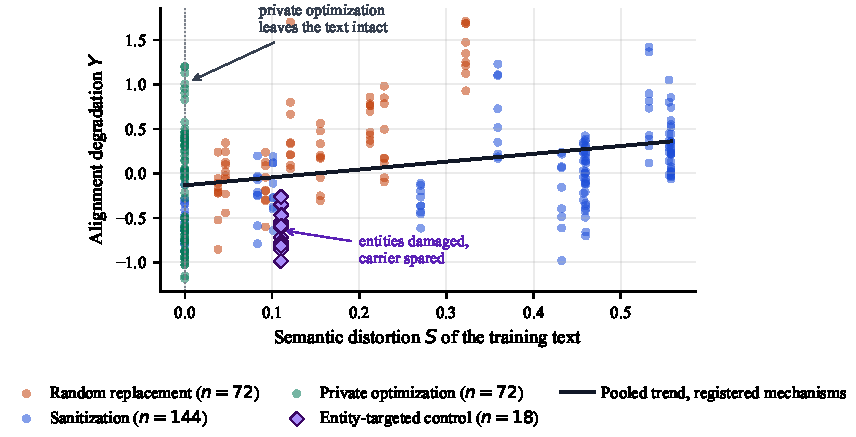
\includegraphics[width=\linewidth]{pathway.pdf}
  \caption{\textbf{Degradation follows distortion, across mechanisms on incomparable privacy scales.} One point per adapter,
  the line an unadjusted trend over the registered mechanisms.
  Private optimization is the vertical cluster at $S \approx 0$,
  leaving the text intact.
  The entity-targeted control sits $0.60$ below the trend,
  which is what identifies the split of \S\ref{sec:carrier}.}
  \label{fig:pathway}
\end{figure}

The level slopes are $-0.128$,
$+0.330$ and $-0.023$ for replacement,
sanitization and private optimization text-side,
and $-0.207$,
$+0.325$ and $-0.005$ generation-side.
The largest of them,
$0.330$,
sits well below $|c| = 0.647$,
so $|c| > |b_m|$ holds for every mechanism under both measurements and the dominance claim is supported.
For private optimization the level slope is $-0.023$ ($\mathrm{SE}\ 0.041$),
so tightening $\varepsilon$ sixteenfold from $16$ to $1$ leaves measured degradation where it was.
Distortion identifies $c$ on its own:
dropping the level term takes the VIF from $8.07$ to $2.08$ and gives $\hat c = +0.403$ ($\mathrm{SE}\ 0.041$, $p < 10^{-21}$),
so the coefficient is large and precisely identified under either specification.

\subsection{\label{sec:carrier}The carrier matters more than the entities}
Splitting distortion reverses the intuition that what privacy costs is the damage done to the sensitive spans themselves.
Within the uniform mechanisms the entity and carrier components are collinear at $r = 0.991$,
inflating variance by a VIF of $58.4$,
which leaves the split unidentified within that family.
The entity-targeted control breaks the collinearity by occupying a region of the distortion space that the uniform mechanisms leave empty,
and gives
\begin{equation}
  \hat c_{\text{carrier}} = +1.83, \qquad \hat c_{\text{entity}} = -0.72 .
  \label{eq:split}
\end{equation}
The model's alignment lives in the ordinary language around the sensitive content,
rather than in the content itself.

\begin{figure}[t]
  \centering
  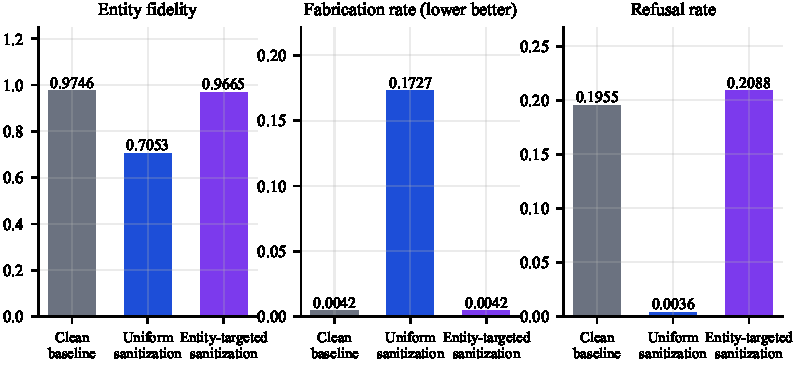
\includegraphics[width=0.66\linewidth]{carrier.pdf}
  \caption{\textbf{At matched entity displacement,
  sparing the carrier preserves fidelity,
  grounding and refusal.} Uniform and entity-targeted sanitization at $\varepsilon = 1$ on the entity-rich dataset,
  against the non-private baseline.
  Both displace entities equally ($S_{\text{entity}} = 0.669$ against $0.671$);
  they differ only in whether the carrier survives.
  Uniform sanitization takes refusal from $0.196$ to $0.004$,
  while the targeted variant leaves it at $0.209$.}
  \label{fig:carrier}
\end{figure}

The outcome gap is the largest single contrast in the study (Table~\ref{tab:targeted}).
At matched entity damage the targeted variant tracks the clean baseline:
fidelity $0.967$ against a baseline $0.975$ and a uniform value $0.705$;
fabrication $0.0042$,
identical to the baseline,
against $0.173$;
refusal $0.209$ against a baseline $0.196$,
where uniform sanitization gives $0.004$.
Uniform sanitization spends most of its behavioral cost on language that carries no private content at all.
The targeted variant is designed to identify the decomposition,
and it does so from a between-family contrast at two budgets;
turning it into a mechanism with a stated guarantee is the natural follow-on.

\subsection{\label{sec:cliff}Sanitization damages alignment at a threshold}
The sanitization budget does its damage in a single step (Figure~\ref{fig:threshold}, \apx{additional}).
Text-side $S$ holds constant to within $0.003$ across $\varepsilon \in [0.5, 3]$ on both datasets,
then collapses between $\varepsilon = 4$ and $6$ and reaches zero by $\varepsilon = 12$.
Four of the eight registered levels therefore sit on a plateau where the mechanism's output is statistically indistinguishable across budgets.
The registered equivalence tests confirm both halves of that shape.
Between the strictest and the loosest plateau setting,
instruction following and the truthfulness margin are equivalent ($p = 0.0001$ and $0.007$),
so the prediction holds on two of three metrics,
entity fidelity sitting outside the margin at $p = 0.064$.
Between the loosest plateau setting and the first past the transition,
all three metrics separate cleanly,
with TOST $p$ above $0.85$ throughout:
the plateau is real and bounded.
The useful design question is which side of the transition a deployment lands on,
rather than where inside the strict region it sits.

\subsection{\label{sec:mediation}The damage runs through fabrication}
Distortion degrades alignment through a specific channel:
it makes the model invent.
Fitting the mediation distortion $\to$ fabrication $\to$ degradation~\citep{imai2010general},
with the outcome taken as instruction following and truthfulness only so the mediator stays outside it,
a unit of distortion raises fabrication by $1.14$ standard deviations.
Conditioning on fabrication drops the direct effect from $+0.518$ to $+0.269$,
leaving an indirect effect of $+0.250$ (bootstrap $95\%$ CI $[+0.173, +0.339]$),
about $48\%$ of the total.
The behavioral end of that chain is the refusal collapse of Figure~\ref{fig:carrier}:
perturbation degrades the language in which a refusal is expressed,
and the model stops producing one.

\subsection{\label{sec:scope}Robustness and scope}
The result reproduces under a second encoder,
under composition of the two mechanisms,
and at four times the model size.
An architecturally unrelated encoder gives $\hat c = +0.608$ and $+0.548$ against $+0.647$ and $+0.543$.
Composing the mechanisms over $72$ adapters costs $+0.306$ summed over the capability probes,
against $+0.372$ for exact additivity and $+0.258$ for the more damaging mechanism alone,
so the two penalties largely stack.
A two-point scale check at $8$B over $62$ adapters gives $\hat c = +0.376$ ($\mathrm{SE}\ 0.189$, $p = 0.052$),
so the pathway survives a fourfold increase in model size,
attenuated on the reduced grid a scale check can afford.

Three boundary conditions delimit the claims.
Leakage sits below the detection floor of our probe,
with record-level rates of $0.0115$ for base models,
$0.0133$ for the non-private baselines and $0.0033$--$0.0047$ across every mechanism,
so the privacy side of the trade rests on the formal guarantees -- as it does in the deployments these mechanisms are built for.
On the registered text-side measurement the effect is invariant to entity density,
so the second dataset replicates the first rather than moderating it;
the generation-side measurement carries a dataset interaction of $+0.153$ against a main effect of $0.405$ (\apx{additional}).
And the fidelity probe is exact on the entity-rich dataset,
where gold spans define it,
while on the entity-poor dataset it carries a seed spread of $0.13$--$0.23$ and the extraction task itself becomes partly unlearnable under the uniform mechanisms,
so the entity-rich estimates carry the fidelity conclusions (\apx{additional}).

\section{\label{sec:discussion}Discussion}
What privacy costs is a cost of semantic damage.
It is distributed unevenly across the kinds of text a mechanism can damage,
and therefore at least partly avoidable by choosing what to damage.

\textbf{Stop tuning the budget and start measuring the text.}
The private optimizer's budget is inert over the range we studied,
so private training carries a fixed penalty that arrives with the mechanism and can be budgeted for once,
and half of the registered sanitization levels are behaviorally identical.
A practitioner who wants to predict what a mechanism will cost should measure what it did to the text,
rather than read its budget.

\textbf{Aim the mechanism at the spans that are sensitive.}
Uniform sanitization at a strict budget leaves refusal at $0.004$ against a baseline of $0.196$,
because the perturbation degraded the language in which a refusal is expressed.
Sparing the carrier restores refusal to its baseline level at matched entity displacement.
The targeted variant is a direction with a clear next step:
it identifies the decomposition on one dataset at two budgets,
and stating the guarantee a span-targeted mechanism provides is the question that turns it into a deployable method.

\textbf{Where the measurements stop.}
Leakage sits below our probe's detection floor at this scale,
so the privacy half of the trade rests on the formal guarantees,
and a sharper extraction attack would put a measured number on it.
We adapt by supervised fine-tuning rather than preference optimization~\citep{ouyang2022training, rafailov2023direct},
we intervene at adaptation time and leave pre-training open,
where factuality suffers more~\citep{ramesh2026privacyhallucination},
and our models span $1$--$2$B parameters,
where the $8$B check finds the pathway attenuated but present.
The natural next step follows from the asymmetry:
a non-uniform noise allocation sparing the directions that carry instruction-following behavior,
and composing \textit{targeted} sanitization with the private optimizer.
Richer notions of meaning than one encoder's,
such as semantic entropy~\citep{farquhar2024detecting},
would enter the same frame as alternative measurements of one latent quantity.

Meaning carries the effect:
the shared coefficient is $0.65$ text-side and $0.54$ on generations against a pre-registered minimum of $0.10$,
and it exceeds every level slope.
What privacy costs alignment is the semantic damage the mechanism did to the text,
and more precisely \textit{which} text it changed.

\printbibliography

\section*{Contributions}
Fang Liu proposed the research idea and the framing of privacy-induced alignment degradation as a question about distinct causal pathways,
and supervised the work.

Dmitry Scherbakov is responsible for the work reported here:
concrete hypotheses and analysis plan,
experimental implementations of perturbation mechanisms,
training loops and evaluations,
analysis,
and the manuscript.

The work was carried out by Dmitry Scherbakov during the Skoltech Summer School in Machine Learning (SMILES) 2026.

\section*{Acknowledgements}
We want to thank Skolkovo Institute of Science and Technology for providing compute resources allocation.

\section*{LLM Usage}
LLMs were used as assistive tools in the preparation of this work,
in four ways:
searching the literature and suggesting related work for the authors to read and verify,
reviewing the source code,
checking papers for spelling,
syntax and factual correctness,
and assembling figures and tables into \LaTeX{} form from values,
produced by the analysis scripts.


\appendix
\section{\label{apx:contrib}Summary of contributions}
What the paper contributes,
in the order the body develops it:

\begin{itemize}
  \item A design that makes the semantic and non-semantic pathways separately estimable,
  by measuring distortion on a common scale across mechanism families and including a distorting mechanism that carries no privacy guarantee.
  \item A pre-registered target quantity,
  minimum effect size and exclusion rule,
  committed before the main pass,
  with every deviation from it reported.
  \item A judge-free evaluation suite.
  No outcome in this paper is scored by a language model,
  which matters when the quantity under study is alignment and any model-based verifier would inherit the property being measured.
  \item Evidence that measured distortion is what predicts alignment degradation,
  dominating the nominal budget,
  which within the private optimizer is inert over the range studied.
  \item A decomposition of distortion into entity and carrier components,
  identified by an entity-targeted control,
  showing that the carrier dominates -- with the corollary that targeting a privacy mechanism at the content that is sensitive is much cheaper than sanitizing uniformly.
  \item A methodological result for replications:
  half of the sanitization budget levels form a behavioral plateau whose transition is locatable from distortion alone before any training,
  and a denser level encoding trades identifying variation for coverage.
\end{itemize}

\section{\label{apx:privacy}Privacy preliminaries}
The two mechanism families of \S\ref{sec:mech} state their guarantees over different spaces,
and that difference is what fixes the design of \S\ref{sec:design}.
This appendix gives the definitions those guarantees use,
states what each mechanism in the grid satisfies,
and relates the sanitization budget to the distortion axis the paper regresses on.

\begin{definition}[$(\varepsilon, \delta)$-differential privacy]
  \label{def:dp}
  A randomized mechanism $\mathcal{M} \colon \mathcal{D} \to \mathcal{R}$ satisfies $(\varepsilon, \delta)$-differential privacy if for every pair of neighboring datasets $D \simeq D'$ and every measurable $E \subseteq \mathcal{R}$,
  \begin{equation*}
    \Pr[\mathcal{M}(D) \in E] \le e^{\varepsilon} \Pr[\mathcal{M}(D') \in E] + \delta .
  \end{equation*}
\end{definition}
The pure case $\delta = 0$ is due to \citet{dwork2006calibrating},
and \citet{dwork2014algorithmic} give the standard development of the relaxation used here.
Throughout,
$D \simeq D'$ means the two datasets differ in one training example,
so the guarantee is example-level over the adaptation set:
one instruction row is the protected unit.

\begin{definition}[R\'enyi differential privacy]
  \label{def:rdp}
  For $\alpha > 1$,
  $\mathcal{M}$ satisfies $(\alpha, \rho)$-R\'enyi differential privacy if $\mathrm{D}_{\alpha}\!\left(\mathcal{M}(D) \,\|\, \mathcal{M}(D')\right) \le \rho$ for every $D \simeq D'$,
  where $\mathrm{D}_{\alpha}$ is the R\'enyi divergence of order $\alpha$.
\end{definition}
R\'enyi differential privacy (RDP) composes additively in $\rho$ over a sequence of releases,
and an $(\alpha, \rho)$ guarantee converts to $\left(\rho + \log(1/\delta)/(\alpha - 1),\, \delta\right)$-DP for any $\delta \in (0, 1)$~\citep{mironov2017renyi}.
Both properties are why the accounting in this paper is carried in $\rho$ and converted once at the end.

\begin{definition}[Metric differential privacy]
  \label{def:metricdp}
  Let $(\mathcal{X}, d)$ be a metric space of inputs.
  A mechanism $\mathcal{M} \colon \mathcal{X} \to \mathcal{R}$ satisfies $\varepsilon d$-privacy if for every $x, x' \in \mathcal{X}$ and every measurable $E \subseteq \mathcal{R}$,
  \begin{equation}
    \Pr[\mathcal{M}(x) \in E] \le e^{\varepsilon d(x, x')} \Pr[\mathcal{M}(x') \in E] .
    \label{eq:metricdp}
  \end{equation}
\end{definition}
Definition~\ref{def:metricdp} generalizes Definition~\ref{def:dp} by letting the admissible likelihood ratio grow with the distance between inputs~\citep{chatzikokolakis2013broadening},
which is what makes it applicable to text:
two words that are far apart in an embedding space are allowed to be distinguishable,
while nearby words are not.
Inputs carrying a natural geometry are what motivate the definition,
and its location instance,
geo-indistinguishability,
has been used to ask of a downstream prediction task the question this paper asks of text:
how much utility the guarantee costs the released object~\citep{liu2021privacy}.

\paragraph{Private optimization.}
DP-SGD clips each per-example gradient to $L_2$ norm $C$,
sums the clipped gradients over a lot drawn by Poisson sampling at rate $q$,
adds $\mathcal{N}(0, \sigma^2 C^2 I)$ and averages~\citep{abadi2016deep}.
The additive noise is the Gaussian member of a family calibrated to the $\ell_p$ sensitivity of the released quantity,
whose scale requirement at a given $(\varepsilon, \delta)$ is characterized by \citet{liu2019ggm}.
Each step is an instance of the sampled Gaussian mechanism,
whose R\'enyi divergence bound $\rho_{\mathrm{SGM}}(\alpha; q, \sigma)$ is given by \citet{mironov2019sgm};
over $T$ steps the released parameter sequence satisfies $(\alpha, T \rho_{\mathrm{SGM}}(\alpha; q, \sigma))$-RDP,
which Definition~\ref{def:rdp} converts to the $(\varepsilon, \delta)$ pair reported in \S\ref{sec:mech} at $\delta = 10^{-5}$,
minimizing over $\alpha$.
Our accountant recomputes $\varepsilon$ from the realized $q$,
$\sigma$ and $T$ of each run rather than from their nominal values;
\apx{dpsgd} reports its validation.

\paragraph{Post-processing.}
DP is closed under post-processing:
if $\mathcal{M}$ satisfies Definition~\ref{def:dp} then so does $f \circ \mathcal{M}$ for any $f$ independent of the data.
The released object here is the adapter,
so every quantity the paper computes downstream of it -- generations,
benchmark scores,
refusal rates,
generation-side distortion -- carries the same guarantee,
and the evaluation suite of \S\ref{sec:eval} consumes no budget however many probes it runs.

\paragraph{Sanitization.}
TEM applies the exponential mechanism~\citep{mcsherry2007mechanism} over a word's embedding neighborhood,
and satisfies \eqref{eq:metricdp} for one replaced word with $d$ the Euclidean metric on the GloVe embedding space,
the support truncated to a ball around the input and mass beyond the threshold going to a fallback symbol~\citep{carvalho2021tem};
it sits in the line of embedding-space text mechanisms opened by \citet{feyisetan2020privacy} and \citet{yue2021differential}.
The unit of the guarantee is a single word,
so a document of $n$ covered tokens composes to $n \varepsilon$ in the worst case,
and the guarantee covers the vocabulary the embedding spans.
Tokens outside that vocabulary are released unchanged,
which is the asymmetry \S\ref{sec:mech} uses:
at matched nominal privacy the two data-side mechanisms damage entities by different amounts,
and \eqref{eq:model} is identified from that gap.

\paragraph{Why the two budgets do not share a scale.}
The $\varepsilon$ of Definition~\ref{def:dp} and the $\varepsilon$ of Definition~\ref{def:metricdp} differ in three places at once.
They quantify over different neighboring relations,
one example against one word.
They constrain different released objects,
a sequence of parameter iterates against a sequence of token releases.
And they compose over different units,
optimizer steps against tokens in a document.
A word-level $\varepsilon = 1$ and an example-level $\varepsilon = 1$ therefore bound the likelihood ratio of different experiments,
and no monotone map carries one to the other.
This is the formal content of the statement in \S\ref{sec:design} that the nominal budgets are incomparable across families:
it is why privacy enters \eqref{eq:model} as the level rank $d_i$ within a mechanism,
and why the cross-family comparison runs through $S$,
which is measured in one set of units for every mechanism.

\paragraph{What the distortion axis measures.}
Metric DP writes its bound as $\varepsilon d(x, x')$,
so the guarantee is stated in a distance,
and a mechanism buys indistinguishability by placing mass on points at some distance from its input.
The expected distance between an input and its release is therefore the quantity in which the sanitization guarantee is priced.
The semantic distortion $S$ of \S\ref{sec:design} is an expectation of that form,
taken at document granularity under a sentence encoder rather than at word granularity under the mechanism's own embedding metric,
so the two are related in kind rather than identical as functionals.
What the correspondence supplies is a reason to expect $S$ to track the mechanism's action closely enough to serve as the shared regressor,
which \S\ref{sec:pathway} confirms empirically.
For private optimization the same distance is zero on the training text by construction,
since the text is never touched,
which is why $S$ is measured between generations of the adapted and the base model in that case,
and why private optimization appears in Figure~\ref{fig:pathway} as a vertical cluster at $S \approx 0$.

\section{\label{apx:extended}Extended design and experimental setup}
This appendix carries the formal development and implementation detail compressed out of \S\ref{sec:design} and \S\ref{sec:setup}.

\subsection{\label{apx:extdesign}Design}
Let $\theta_0$ be a small instruction-tuned open-weight LLM.
Each run applies a privacy mechanism $m_i$ at a given strength,
acting on either the adaptation data or the adaptation procedure,
and produces an adapted model.
Each run yields two measurements.
\textbf{Semantic distortion} $S_i$ is the mean cosine distance between sentence embeddings of the original and the rewritten training text;
where the mechanism leaves the text intact,
it is measured between generations of the adapted and the base model on a fixed probe set.
$S$ is computed without reference to the privacy parameter that produced it.
\textbf{Alignment degradation} $Y_i$ is the drop from the same model's non-private baseline on the evaluation suite of \S\ref{sec:eval}.

The two candidate pathways make opposite predictions about what survives conditioning on distortion:
if degradation runs through meaning,
the association between privacy level and $Y$ vanishes once $S$ is held fixed;
if it does not,
a level effect remains at fixed $S$. Splitting the association that way and writing it linearly yields
\begin{equation}
  Y_i = a_{m_i} + b_{m_i} d_i + c S_i + e_i,
  \label{eq:modelext}
\end{equation}
where $d_i$ is the privacy-level rank of run $i$ within its own mechanism,
$a_m$ and $b_m$ are a per-mechanism intercept and level slope,
respectively,
and $e_i$ is the error term.
A random intercept per base model is added to $a_m$.
$Y$,
$d$ and $S$ are z-scored,
so $b_m$ and $c$ are standardized effects on a common scale.
Baseline runs have $Y \equiv 0$ by definition:
they set the zero point and are not regression rows.

Despite the mechanism index on $a_m$ and $b_m$,
\eqref{eq:model} is one regression estimated jointly over all mechanism runs through indicator variables:
seven coefficients fitted in a single pass,
with the per-model random intercept as a mixed-effects term.
The pre-registered cluster-robust correction by model~$\times$~mechanism cell is recorded as a deviation in \apx{deviations}.
Each row activates the intercept and slope of its own mechanism only.
The $S$ column carries no indicator,
so $c$ is shared and pools mechanisms that disagree about how much distortion a given privacy level buys.
Joint estimation puts $\hat c$ and each $\hat b_m$ in one covariance matrix,
so comparing them is a Wald test on linear combinations of coefficients.

The privacy level enters \eqref{eq:model} only through its rank $d_i$.
Within each mechanism the settings are ordered from strictest to loosest,
coded $1$ upward,
and z-scored,
so mechanisms with different numbers of levels enter on the same scale.
The nominal budgets are incomparable across families:
private optimization gives example-level $(\varepsilon, \delta)$-DP~\citep{abadi2016deep},
sanitization word-level metric local differential privacy (LDP)~\citep{chatzikokolakis2013broadening}.
Rank coding rests on the ordering of the settings alone,
which leaves $S$ as the one regressor common to every mechanism.

We state the claim in two stages,
because a shared coefficient can be statistically distinct from zero and still too small to matter.
The first stage fixes a negligibility floor $\Delta = 0.10$ in standardized units,
committed before the main pass together with the primary $S$ metric and the exclusion rules,
and asks whether $|c| \ge \Delta$:
distortion moves alignment by an amount worth acting on.
The value of $\Delta$ is arbitrary and the conclusion does not turn on it;
it marks the point below which an effect is negligible,
so a confidence interval for $c$ contained in $(-\Delta, \Delta)$ settles the first stage the other way,
establishing the practical absence of the semantic pathway by TOST.
The second stage is the substantive one:
$|c| \gg |b_m|$ for every mechanism,
distortion predicting degradation far more strongly than the nominal privacy level,
tested as $|c| > |b_m|$ on the joint covariance of \eqref{eq:model}.

Within a single mechanism $S$ and $\varepsilon$ are correlated by construction,
so no one mechanism separates $b_m$ from $c$. The design produces variation in $S$ at fixed privacy from two sources.
The first is the contrast between families,
which reach comparable privacy with different amounts of semantic damage:
sanitization passes out-of-vocabulary tokens through untouched while random replacement destroys them,
and personally identifiable information (PII) is typically out of vocabulary (\S\ref{sec:mech}).
The second is a non-private control.
If it degrades alignment as much as the private conditions at equal $S$,
semantic damage rather than privacy is the cause;
if it does not,
the residual measures mechanism-specific,
non-semantic effects.
We report VIF for $S$,
falling back to the within-level cross-mechanism contrast,
which is free of $\varepsilon$ -- $S$ confounding.

\subsection{\label{apx:extsetup}Experimental setup}
Here, we describe datasets,
privacy mechanisms,
models and evaluation suite.

\subsection{Datasets}
The text the mechanisms perturb stands in for the sensitive data.
The two datasets differ in \textbf{entity density},
because privacy risk concentrates in names,
numbers and facts,
and the mechanisms treat these tokens differently from common words:
rare tokens occupy sparse regions of embedding space,
so sanitization replaces them with distant,
fact-changing substitutes,
and private optimization suppresses the memorization of exactly such rare sequences.

\paragraph{Entity-rich.}
\texttt{nvidia/Nemotron-PII}~\citep{nvidia2025nemotronpii} is a synthetic dataset of emails,
clinical notes,
forms and free text,
with gold span-level PII annotations.
The gold spans make the entity component of $S$ exact rather than dependent on a noisy named entity recognition model,
and let us measure whether an adapted model reproduces or corrupts specific entities.
We restrict to the biomedical domains for simplicity.
The mechanisms perturb text without regard to domain,
so one domain suffices to study them and a broader set would add cost without changing what we measure.
We keep records with at least one parsable span.

Each document is rendered once into an instruction example,
reused by every condition,
under one of three templates sampled per record:
extract a labeled entity,
draft a document of the given type and domain,
or classify the document type.
The training set is $16{,}384$ rows.
A further $375$ records are held out for the entity-fidelity probe,
disjoint \textit{by source document} rather than by rendering,
since one document appears under several renderings and splitting on rows would leak.
Another $375$ are sampled from the training rows for the leakage probe;
these are not held out,
because the probe asks whether training memorized them.

\paragraph{Entity-poor.}
A fixed subset of Alpaca~\citep{taori2023alpaca} of the same size:
generic assistant tasks with few named entities or numbers,
and the standard small instruction-tuning dataset,
which keeps results comparable to prior work.
Gold spans define the entity and carrier components of $S$,
so those two components are reported on the entity-rich dataset,
and the entity-poor dataset carries the composite $S$ alone.
Dataset construction and perturbation run as a single pass emitting both datasets together,
so the perturbed datasets are matched on both sides of the entity-density contrast.

\subsection{\label{apx:mech}Privacy mechanisms}
The registered grid has four conditions:
a non-private baseline,
a non-private distorting control,
and two mechanisms carrying formal guarantees.

\paragraph{No privacy (baseline).}
Standard LoRA fine-tuning on the clean dataset,
defining the zero point of both $Y$ and $S$.

\paragraph{Random token replacement.}
Text is tokenized on whitespace,
numbers and identifiers included,
and each token is independently replaced with probability $p \in \{0.05, 0.15, 0.30, 0.50\}$ by a token drawn uniformly from its own dataset vocabulary.
A higher rate is the stricter setting,
so the rank order is reversed relative to the $\varepsilon$-indexed mechanisms.
It carries no privacy guarantee;
its purpose is to vary distortion -- entity distortion in particular,
since whitespace tokenization exposes identifiers -- independently of any privacy budget.

\paragraph{Sanitization.}
We use TEM~\citep{carvalho2021tem} rather than a plain SanText-style exponential mechanism over the full vocabulary~\citep{yue2021differential}.
TEM restricts the candidate set to words within a distance threshold and folds the remaining mass into a truncation symbol,
avoiding the plain mechanism's low-probability substitutions drawn from arbitrarily distant words.
For a word $x$ with embedding $e_x$,
the near set is $N = \{w : \lVert e_x - e_w \rVert_2 \le \gamma\}$ and the far set $F = V \setminus N$,
with utility $u(w) = -\lVert e_x - e_w \rVert_2$ and a truncation symbol $\bot$ of utility $u(\bot) = -\gamma + \tfrac{2}{\varepsilon} \ln|F|$;
a substitute is drawn from $N \cup \{\bot\}$ with probability proportional to $\exp(\tfrac{\varepsilon}{2} u)$,
and if $\bot$ is drawn a word is emitted uniformly from $F$. We use word-level $\varepsilon \in \{0.5, 1, 2, 3, 4, 5, 6, 12\}$ and $\gamma = 5.0$,
sampling per token occurrence but memoizing the per-word-type distribution across occurrences and datasets,
which makes the mechanism tractable over a $400$k-word vocabulary.

Word distances come from pre-trained GloVe 6B.300d vectors~\citep{pennington2014glove}.
Perturbation runs once and its output is consumed by all three models;
deriving the metric from a base model's own embedding matrix would make the sanitized dataset model-specific and entangle $S$,
the pooled regressor on which the design rests,
with model identity.
GloVe is also a \textit{word}-level vocabulary,
matching the units in which the entity component of $S$ is defined,
where a mechanism over BPE tokens would fragment entities across sub-tokens.
Out-of-vocabulary passthrough follows from the same choice:
medical record numbers,
phone numbers and email addresses are out of vocabulary in GloVe,
so TEM leaves them intact and \textit{preserves} literal entities where random replacement destroys them at matched nominal privacy.
That asymmetry is the identification strategy of \S\ref{sec:design},
and subword vectors such as fastText would remove it.

Both data-side mechanisms rewrite only the content fields of each instructionized example,
leaving the instruction template intact:
the instruction is a fixed task specification rather than sensitive data,
and perturbing it corrupts what the model is asked to do instead of the signal the mechanism acts on.
Perturbed rows keep the original schema and gold-span offsets,
so entity-level distortion is computed by joining each perturbed row to its clean counterpart on the example identifier.

\paragraph{Private optimization.}
DP-SGD~\citep{abadi2016deep} is applied to the LoRA parameters at example-level $\varepsilon \in \{1, 4, 8, 16\}$ with $\delta = 10^{-5}$.
Lots are drawn by Poisson subsampling,
each example included independently with probability $q = B/N$.
This is not interchangeable with shuffled fixed-size minibatches:
the amplification result the accountant applies is proved for Poisson sampling~\citep{mironov2019sgm},
and under shuffled batches the reported $\varepsilon$ would misstate the mechanism that was run.
Per-example gradients are clipped to $\lVert g \rVert_2 \le C$ and accumulated in fp32,
Gaussian noise $\mathcal{N}(0, (\sigma C)^2)$ is added to the sum,
and the result is divided by the \textit{configured} lot size rather than the number of examples drawn,
as Poisson sampling requires.
The private loop is written directly against the adapter parameters,
but privacy accounting is delegated to an established implementation:
a numerical inversion for the $\varepsilon \mapsto \sigma$ calibration,
and a R\'enyi accountant~\citep{mironov2017renyi} for the realized $\varepsilon$,
recomputed at the chosen $\sigma$ over the actual step count and logged as the reported guarantee.
An error in a training loop shows up in the loss;
an error in a hand-vendored accountant silently under-reports $\varepsilon$.
\apx{dpsgd} gives the implementation details,
the end-to-end validation of the calibration,
and the pitfalls specific to this branch.
In the registered grid the mechanisms are kept separate:
the private branch trains only on clean text.
A post-hoc block lifts that restriction (\S\ref{sec:scope}).
A post-hoc block lifts that guard to measure their interaction (\S\ref{sec:scope}).

\paragraph{Entity-targeted sanitization (post-hoc control).}
This variant was added after the main fit to separate the entity and carrier components of $S$,
which uniform sanitization moves together (\S\ref{sec:carrier}).
It applies TEM to the gold entity spans alone -- resampling each distinct entity once and substituting it at every occurrence -- and leaves the carrier text verbatim.
It runs at two budgets on the entity-rich dataset only,
since the targeting requires the gold spans.
At matched entity displacement it inflicts a fraction of the carrier damage that uniform sanitization does,
isolating the two components the uniform mechanism confounds.

\subsection{Models and adaptation}
We use three dense open-weight instruction-tuned models in the $1$ -- $2$B range:
Qwen3-1.7B~\citep{yang2025qwen3},
Llama-3.2-1B-Instruct~\citep{grattafiori2024llama},
and Falcon3-1B-Instruct~\citep{falcon3}.
The size is set by the grid:
with $324$ adapters to train and evaluate,
each must cost tens of GPU-minutes for the design to remain affordable.
Three \textit{families} rather than three checkpoints of one family let the per-model random intercept absorb base-model idiosyncrasy;
the claims of \S\ref{sec:design} require variation across pretraining recipes and tokenizers.
All three expose the same query and value projections,
keeping the adapter target set identical across conditions.
We exclude the newest hybrid small models -- gated linear attention with sparse mixture-of-experts -- since per-example gradient computation is awkward there and an accounting error on a novel architecture would invalidate the entire private column.

Every condition uses the same adaptation procedure:
LoRA~\citep{hu2022lora} with rank $16$,
$\alpha = 32$,
adapters on the query and value projections,
no dropout and no bias terms,
the base model loaded in bf16 and frozen,
and loss taken on completion tokens only using the same chat-template call the evaluation harness uses.
This gives $3{,}211{,}264$ trainable parameters.
Sequences are truncated at $2048$ tokens and training runs for $3$ epochs at a lot size of $256$,
with a warmup--stable--decay learning-rate schedule~\citep{hu2024minicpm} specified in \textit{fractions} of total steps,
so its shape is identical in every cell.
The conditions differ only in which dataset they consume,
except the private one,
which additionally runs the private loop,
gated on the presence of a target $\varepsilon$ rather than on a global flag.

Holding the procedure fixed leaves the mechanism as the only varying factor,
a precondition for \eqref{eq:model} to attribute differences in $Y$ to $S$ and the privacy level rather than to training hyperparameters.
The fixed learning rate carries a cost,
since private conditions often prefer a higher rate than clean ones and the shared value was tuned on the clean condition.
We measured it:
the tuned rate improves the private mechanism as well,
at every budget tested.
\apx{calib} reports the calibration runs,
the seed-noise floor that terminates them,
and two settings whose response is flat.

Epochs are held at $3$ because they affect privacy:
$\sigma$ is calibrated over the total step count,
so more epochs mean more composition and a noisier private mechanism at the same $\varepsilon$.
Training longer would give the non-private conditions more optimization and the private mechanism both more optimization and more noise,
an asymmetry that would enter $\hat b_m$ and confound the effect the regression measures.
Lot size is free of this coupling:
the private branch performs one backward pass per \textit{example},
so total work is independent of $B$,
and lot size is the parameter used to raise the gradient signal-to-noise ratio (\apx{dpsgd}).

\subsection{\label{apx:eval}Evaluation}
Every component of $Y$ is judge-free:
no LLM judge enters the measurement chain,
so the dependent variable is independent of any judge model's own alignment properties.
Decoding is greedy and capped at a fixed number of new tokens,
the same cap in every condition.

\paragraph{Truthfulness.}
TruthfulQA~\citep{lin2022truthfulqa} MC1 and MC2 on the validation split.
We score each option by the summed token log-probabilities of the option conditioned on the question prompt,
giving a likelihood over the fixed options.

\paragraph{Instruction following.}
IFEval~\citep{zhou2023instruction},
whose prompts carry programmatically verifiable constraints;
we report prompt-level and instruction-level accuracy using the reference verifiers.

\paragraph{Entity fidelity (hallucination).}
The model is asked to extract a gold-annotated entity from each of the $375$ held-out records,
with the requested label drawn deterministically per record.
Responses are scored against the gold spans into three exclusive outcomes:
\texttt{correct},
\texttt{corrupted} (every returned value occurs somewhere in the record, but the set is incorrect),
and \texttt{fabricated} (some returned value does not occur in the record at all, or nothing is returned).
The distinction separates the two pathways:
corruption indicates a model trained on distorted entities,
fabrication one that lost grounding entirely.

\paragraph{Refusal.}
Refusal is measured on the $520$ harmful instructions of AdvBench~\citep{zou2023universal} and on XSTest~\citep{rottger2024xstest},
whose $450$ prompts divide between benign requests phrased so as to look alarming and genuinely unsafe ones.
A response counts as a refusal when one of a fixed list of refusal phrases occurs in its first $120$ characters,
the same rule in every condition,
which keeps the measurement judge-free.
The two suites together separate a model that has become discriminating from one that declines whatever it is asked.
Refusal is reported alongside $Y$ and stays outside it (\apx{refusal}).

\paragraph{Entity leakage (memorization).}
Leakage is reported alongside $Y$ and stays outside it.
For the $375$ records that \textit{were} in the training set,
the model is shown the first half of the document and asked to continue it verbatim;
we count how many gold entities in the withheld second half are reproduced.
This is an extraction attack in miniature~\citep{carlini2021extracting} and serves as a manipulation check:
a mechanism whose leakage matches the baseline has not delivered the privacy whose alignment cost the paper measures.

\subsection{Semantic distortion}
The primary measure,
fixed before the main pass,
is the embedding distance of \S\ref{sec:design},
computed with \texttt{BAAI/\allowbreak bge-base-\allowbreak en-v1.5}~\citep{xiao2024cpack} as the sentence encoder.
$S$ is additionally reported as two components:
$S_{\mathrm{ent}}$,
the fraction of named entities and numbers not preserved between original and perturbed text,
defined against gold spans,
so reported on the entity-rich dataset;
and $S_{\mathrm{gen}}$,
the residual embedding drift after masking entities.
We test whether $S_{\mathrm{ent}}$ drives truthfulness and hallucination degradation while $S_{\mathrm{gen}}$ drives instruction-following degradation,
by refitting \eqref{eq:model} with the two components in place of $S$. Because the embedding-based components rest on a single encoder,
every distortion score is recomputed with a second,
unrelated encoder (\texttt{all-\allowbreak MiniLM-\allowbreak L6-v2}~\citep{wang2020minilm, reimers2019sbert}) as a robustness check;
the primary measure was fixed in advance so that it could not be selected after the results were visible.
The entity component is a token-membership rate rather than an embedding distance,
so it is invariant to that choice by construction.

\subsection{Experiment coverage}
Random replacement has four rates and private optimization four budgets;
sanitization has eight,
whose cost in collinearity exceeded its gain in coverage (\apx{deviations}).
Together the mechanisms give $17$ conditions per model on the entity-poor dataset:
the non-private baseline,
four rates of random replacement,
eight budgets of sanitization,
and four budgets of private optimization.
The entity-rich dataset adds two budgets of the entity-targeted control,
for $19$.
Across three base models and three seeds this is $153$ and $171$ adapters respectively,
$324$ in total,
of which $288$ enter \eqref{eq:model}:
the sixteen registered mechanism conditions per dataset.
The baseline sets the zero point,
and the entity-targeted control is a post-hoc addition analyzed separately (\S\ref{sec:carrier}).
Counting calibration,
the sensitivity blocks of \apx{sensitivity},
and repeated runs,
$444$ training runs were executed.
The three seeds supply the within-condition variance,
so every reported point carries an error bar.

\section{\label{apx:calib}Hyperparameter calibration}
All tuning was performed on a held-out seed,
$99$,
disjoint from the grid seeds $0$--$2$;
on the clean condition only;
and applied unchanged to every condition.
Tuning per condition would have introduced exactly the confound the shared recipe exists to prevent.
The runs below are calibration measurements.

\paragraph{Peak learning rate.}
A lot size of $256$ makes $3$ epochs $192$ optimizer steps instead of $3072$,
so the rate inherited from a $B{=}16$ configuration is far too small:
at $2\times10^{-4}$ the clean condition reaches validation loss $0.9648$ against $0.8250$ at $B{=}16$,
and $6\times10^{-4}$ recovers only to $0.8700$.
Table~\ref{tab:lr} scans the peak rate on all three models.
We adopt $3.2\times10^{-3}$ for all three rather than one value per model,
because the data do not separate them.

\begin{table}[h]
\centering
\begin{tabular}{@{}lccc@{}}
\toprule
Peak LR & Qwen3-1.7B & Llama-3.2-1B & Falcon3-1B \\
\midrule
$1.0\times10^{-3}$ & 0.8425 & 1.0095 & 0.9402 \\
$2.0\times10^{-3}$ & 0.8186 & 0.9868 & 0.8931 \\
$\mathbf{3.2\times10^{-3}}$ & \textbf{0.8122} & \textbf{0.9809} & \textbf{0.8724} \\
$5.0\times10^{-3}$ & 0.8141 & 0.9876 & -- \\
$8.0\times10^{-3}$ & 0.8484 & -- & -- \\
\bottomrule
\end{tabular}
\caption{Final validation loss on the clean condition,
lot size $256$,
$3$ epochs,
calibration seed $99$.
The optimum is bracketed on both sides for Qwen and Llama;
the Falcon cell at $8\times10^{-3}$ was stopped once it trailed its $3.2\times10^{-3}$ counterpart at epoch~1.}
\label{tab:lr}
\end{table}

\paragraph{Where the search stops.}
Three seeds of the \textit{same} recipe differ at epoch $0$ by $0.0067$ ($0.8865$, $0.8886$, $0.8932$).
The gap between $3.2\times10^{-3}$ and $5\times10^{-3}$ in Table~\ref{tab:lr} is $0.0019$,
a quarter of that spread,
so the two settings are indistinguishable and any further point in this range would measure seed noise.
The same floor bounds what the design needs to resolve elsewhere:
the gap in validation loss between the non-private and private conditions at fixed learning rate is about $0.315$,
roughly $47\times$ the seed spread,
so the quantity the regression must estimate sits far above the noise level at three seeds per cell.

\paragraph{The tuned rate transfers to the private mechanism.}
Tuning on the clean condition carried the risk that a $16\times$ increase in learning rate would diverge against gradients clipped to nearly direction-only.
It does the opposite.
At $\varepsilon = 8$ the loss improves from $1.2808$ at $2\times10^{-4}$ to $1.1335$ at the tuned rate;
at $\varepsilon = 1$,
from $1.3712$ to $1.2532$ after one epoch.
The perturbed conditions gain as well ($2.8927 \to 2.7212$ after one epoch at $p{=}0.30$),
with no divergence and no NaN in any cell,
so no per-mechanism learning rate is required.

\paragraph{Two settings with flat response.}
Both were live hypotheses that would otherwise be re-proposed.
\textit{Clipping bound.} At the tuned rate and $\varepsilon = 8$,
$C = 0.5$ gives $1.1857$,
$C = 1.0$ gives $1.1859$ and $C = 2.0$ gives $1.2045$;
the first two agree to four decimals.
The knob is demonstrably live -- the fraction of clipped examples moves $0.684 / 0.645 / 0.432$ across the three -- it does not matter at this scale,
so $C = 1.0$ stands.
That fraction also falls as the rate rises ($0.773$ at $2\times10^{-4}$ against $0.645$ at $3.2\times10^{-3}$, both at $\varepsilon = 8$),
since larger steps shrink the gradients;
the two interact,
which is why $C$ was re-probed at the new rate rather than carried over.
\textbf{Decay onset.} Starting the cosine at $1.14$ epochs instead of $1.5$ changes Llama's final validation loss from $0.9809$ to $0.9775$ and Qwen's epoch-$0$ loss from $0.8865$ to $0.8856$.
Both sit below the resolution floor.

\paragraph{Sequence length.}
Truncation at $2048$ tokens is inexpensive and fixes real data loss:
at $1024$,
$50$ rows have prompts that fill the window entirely and $103$ completions are cut short;
at $2048$ those counts are $2$ and $0$. Doubling again to $4096$ drops nothing further while doubling activation memory,
which is the binding constraint in the private branch.

\paragraph{Validation loss serves as a diagnostic.}
An optional fixed-seed holdout logs token-weighted validation loss once per epoch,
splitting on a fixed generator rather than on the run seed so that every condition and seed holds out the same rows.
It is disabled for the main grid.
Each perturbed condition validates against its own perturbed distribution,
so the levels are incomparable by construction -- $0.96$,
$3.15$ and $4.81$ for the clean condition,
random replacement at $p{=}0.30$ and sanitization at $\varepsilon{=}3$ under otherwise identical settings.
That reflects a different target.
Within one fixed dataset it remains a valid training diagnostic,
which is how it is used above.
With the holdout disabled,
the grid trains on all $16{,}384$ rows and the privacy guarantee covers the whole dataset.


\section{\label{apx:dpsgd}DP-SGD implementation}
This appendix covers the accountant validation,
the precision and lot-size choices,
the per-example gradient implementation,
and the pitfalls specific to the private branch.

\paragraph{Accountant validation.}
For target $\varepsilon = 8$ at $q = 0.01$,
$100$ steps and $\delta = 10^{-5}$,
the calibration returns $\sigma \approx 0.50$ and the recomputed guarantee is $\varepsilon \approx 7.995$.
At $3$ epochs and $B = 16$ over $16{,}384$ rows ($3072$ steps, $q \approx 9.77 \times 10^{-4}$) the calibration gives $\sigma \approx 0.437$ at $\varepsilon = 8$ and $\sigma \approx 0.864$ at $\varepsilon = 1$. Re-running the accounting with R\'enyi orders up to $1024$ reproduces the realized $\varepsilon$ to three decimals at both budgets,
so the default order grid costs no utility.

\paragraph{Numerical precision.}
The lot gradient is accumulated into an fp32 buffer and cast back to bf16 only at gradient assignment.
Performing the accumulation and the noise draw in bf16 instead rounds much of the calibrated noise away,
and the run then reports an $\varepsilon$ it does not deliver.

\paragraph{Lot size.}
At a lot size of $16$ the private conditions are severely under-batched.
With $\sigma = 0.437$ and $d = 3{,}211{,}264$ trainable parameters,
the averaged noise vector has norm $\approx 49$ against a signal of at most $C = 1$:
the update is roughly $98\%$ noise.
Lot size is the only knob that fixes this for free.
Analytically,
$\sigma$ grows only about $7\%$ per doubling of $B$,
so $B = 256$ at $3$ epochs yields $12.1\times$ the gradient signal-to-noise ratio at $1.0\times$ the cost,
whereas $B = 256$ at $6$ epochs yields \textit{less} ($11.3\times$) at $2.0\times$ the cost.
The measured ratio improved about $7\times$ ($0.010 \to 0.073$ at $\varepsilon = 8$).
Raising the adapter rank instead would have been actively harmful,
since the noise is injected per trainable parameter and more capacity therefore means more noise at the same $\varepsilon$.

\paragraph{Per-example gradients by explicit loop.}
The natural implementation vectorizes per-example gradients with \texttt{torch.func}~\citep{paszke2019pytorch},
and the small adapter parameter count makes that look cheap.
It is not.
There is no batching rule for the fused FlashAttention~\citep{dao2022flashattention} backward kernel,
so the vectorizing transform falls back to a path that materializes the full sequence\,$\times$\,sequence attention matrix per example,
and the branch exhausted memory at $16 \times 2048$ on the grid instance.
Neither a lower LoRA rank nor micro-batching addresses this,
because the vectorization itself is the cost.
The private branch therefore iterates over the lot one example at a time,
clipping in place and accumulating.
This is slower per step but bounded,
and the ratio is structural rather than tunable -- one backward pass per example regardless of lot size -- costing about $2.8\times$ the wall-clock of the non-private mechanism ($97$ against $35$ minutes at $B = 16$).

\paragraph{Lot size variability.}
Under Poisson subsampling the realized lot size varies (at $B = 16$: mean $16$, sd $3.9$, observed range $7$--$30$),
and empty lots are skipped,
which only over-pays privacy.

\paragraph{Two pitfalls specific to the private branch.}
Rows whose prompt fills the context window have every label masked,
so their per-example cross-entropy is NaN;
summed into the lot gradient this contaminates every adapter parameter and yields a garbage checkpoint with only a NaN in the loss log to show for it.
Such rows are dropped before training and counted.
Separately,
dropout is disabled by setting every dropout module's rate to zero rather than by placing the model in evaluation mode:
a live dropout mask would break the per-example determinism the accounting assumes,
while evaluation mode would additionally disable training-mode behavior elsewhere in the network.


\section{\label{apx:additional}Additional results and analyses}
\subsection{\label{apx:sensitivity}Sensitivity to training configuration}
Three configuration blocks were run on the entity-rich dataset,
nine adapters each,
to test whether the flatness of private optimization and the choice of three epochs are properties of the mechanism or of our settings (Table~\ref{tab:sensitivity}).

\begin{table}[t]
  \centering
  \caption{Configuration blocks, entity-rich dataset,
  nine adapters each.
  The grid configuration is clipping bound $1.0$,
  rank $16$,
  three epochs.}
  \label{tab:sensitivity}
  \begin{tabular}{llccc}
    \toprule
    Block & Setting & Fidelity & Instruction & $Y$ \\
    \midrule
    \multirow{3}{*}{Clipping bound}
      & $0.1$  & 0.9303 & 0.2530 & $-0.417$ \\
      & $0.3$  & 0.9300 & 0.2559 & $-0.412$ \\
      & $3.0$  & 0.9260 & 0.2481 & $-0.403$ \\
    \midrule
    \multirow{3}{*}{Adapter rank}
      & $4$    & 0.9417 & 0.2964 & $-0.596$ \\
      & $8$    & 0.9414 & 0.2777 & $-0.547$ \\
      & $32$   & 0.9022 & 0.2138 & $-0.508$ \\
    \midrule
    \multirow{2}{*}{Six epochs}
      & Baseline      & 0.9695 & 0.2627 & -- \\
      & Private optim.& 0.9007 & 0.1717 & $-0.076$ \\
    \bottomrule
  \end{tabular}
\end{table}

\paragraph{The clip is inert.}
Varying the clipping bound from $0.1$ to $3.0$ -- a thirtyfold range spanning both sides of the mean gradient norm -- moves fidelity by $0.004$ and $Y$ by $0.014$.
Together with the budget flatness of \apx{clipping} this says the mechanism's two tuning knobs are both inert at this scale,
which strengthens rather than weakens the clipping-bias account:
when most examples are clipped at every setting ($0.561$--$0.753$ of them),
moving the threshold changes which examples are clipped rather than whether clipping occurs.

\paragraph{Rank is not.}
Adapter rank moves outcomes more than either privacy knob:
instruction following falls from $0.296$ at rank $4$ to $0.214$ at rank $32$,
and $Y$ rises by $0.088$ over the same range.
A larger adapter fits the perturbed data better and is damaged more by it.
Any comparison of private-optimization cost across papers is therefore confounded by adapter capacity unless it is held fixed.

\paragraph{Three epochs against six.}
On clean text six epochs reproduces three to within $0.005$ on fidelity and $0.001$ on instruction following,
so the baseline is saturated.
Under private optimization it is not:
six epochs costs $0.09$ of instruction following relative to the three-epoch runs and raises $Y$ by $0.31$.
Longer private training costs more here,
consistent with accumulated clipping bias rather than with undertraining.

\subsection{Secondary truthfulness measures}
The suite records four truthfulness quantities beyond the primary multiple-choice accuracy (Table~\ref{tab:truthfulqa}).
All are computed on the same $817$ questions.

\begin{table}[t]
  \centering
  \caption{TruthfulQA measures by mechanism,
  averaged over datasets,
  levels,
  models and seeds.
  Normalized variants divide the option log-probability by option length;
  expected calibration error (ECE)~\citep{guo2017calibration} uses ten equal-width confidence bins.}
  \label{tab:truthfulqa}
  \small
  \setlength{\tabcolsep}{4pt}
  \begin{tabular}{lcccccc}
    \toprule
    Mechanism & MC1 & MC1$_n$ & MC2 & MC2$_n$ & Margin & ECE \\
    \midrule
    Base                 & 0.3137 & 0.3639 & 0.4904 & 0.4578 & $-0.9977$ & 0.1672 \\
    Baseline adaptation  & 0.2382 & 0.2782 & 0.3828 & 0.4017 & $-0.9025$ & 0.1636 \\
    Random replacement   & 0.2269 & 0.2711 & 0.3869 & 0.4034 & $-0.7714$ & 0.1428 \\
    Sanitization         & 0.2500 & 0.2862 & 0.4241 & 0.4189 & $-0.6678$ & 0.1343 \\
    Entity-targeted      & 0.2390 & 0.2780 & 0.3833 & 0.4056 & $-0.8177$ & 0.1535 \\
    Private optimization & 0.2331 & 0.2674 & 0.3812 & 0.4018 & $-0.8568$ & 0.1585 \\
    \bottomrule
  \end{tabular}
\end{table}

Three observations.
Length normalization raises MC1 by four to five points uniformly and does not change any ordering.
Adaptation costs about eight points of MC1 and eleven of MC2 relative to the base model,
consistent with the instruction-following loss of \apx{sanity}.
And calibration error \textit{falls} under the text-perturbing mechanisms,
from $0.164$ at the non-private baseline to $0.134$ under sanitization,
in the same direction as the rising margin:
distorted models are less confident and,
on this measure,
better calibrated.
The entity-targeted control sits at $0.154$,
between the baseline and the uniform mechanism,
tracking its intermediate carrier damage.
Whether this is a benefit or an artifact of flattened output distributions is not resolved here.

\subsection{Instruction-level accuracy}
IFEval admits a stricter prompt-level score,
requiring every instruction in a prompt to be satisfied,
and a looser instruction-level score.
Both are recorded;
the primary analysis uses the former.
They move together (Table~\ref{tab:ifevallevels}),
with the instruction-level score running $10$--$11$ points higher throughout and preserving every mechanism ordering,
so no conclusion depends on the choice.

\begin{table}[t]
  \centering
  \caption{IFEval at both granularities,
  averaged over levels,
  models and seeds.}
  \label{tab:ifevallevels}
  \begin{tabular}{llcc}
    \toprule
    Dataset & Mechanism & Prompt-level & Instruction-level \\
    \midrule
    \multirow{3}{*}{Poor}
      & Baseline       & 0.3383 & 0.4543 \\
      & Replacement    & 0.2126 & 0.3218 \\
      & Sanitization   & 0.2249 & 0.3308 \\
      & Private optim. & 0.3178 & 0.4338 \\
    \midrule
    \multirow{5}{*}{Rich}
      & Baseline       & 0.2639 & 0.3750 \\
      & Replacement    & 0.1543 & 0.2513 \\
      & Sanitization   & 0.1993 & 0.3067 \\
      & Entity-targeted& 0.2610 & 0.3713 \\
      & Private optim. & 0.2560 & 0.3688 \\
    \bottomrule
  \end{tabular}
\end{table}

\subsection{Accounting and compute}
The privacy accountant's realized budgets match their targets to three decimals ($0.991$, $3.995$, $7.999$, $15.995$ against nominal $1$, $4$, $8$, $16$),
at noise multipliers of $1.299$,
$0.740$,
$0.581$ and $0.453$ and a mean sampled lot size of $238$.
The delta is fixed below the reciprocal of the dataset size throughout.

The full grid cost approximately $407$ GPU-hours:
$339$ in training -- $33.6$ minutes for a mean non-private cell against $71.0$ for a private one,
the private branch being roughly twice as expensive per cell because per-example gradients are computed by loop rather than vectorised (\apx{dpsgd}) -- $66$ across both evaluation suites,
and under three hours for the single distortion pass over $26$ text variants and $387$ generation sets.

\subsection{Coverage}
The grid completed in full.
The entity-poor dataset contributes $17$ conditions per model -- one non-private baseline,
four levels of random replacement,
eight of sanitization and four of private optimization -- and the entity-rich dataset adds two levels of entity-targeted sanitization for $19$.
Across three base models and three seeds this is $153$ and $171$ adapters,
$324$ in total,
from $444$ training runs;
the excess is the tuning wave of \apx{calib} together with the configuration-sensitivity runs of \apx{sensitivity}.
Every adapter was evaluated on the alignment suite and,
separately,
on the refusal suite,
giving $408$ evaluations of each kind ($405$ adapters plus the three untuned base models).

Semantic distortion was scored on all $26$ perturbed text variants and on $387$ generation sets -- one for every adapter that has a non-private counterpart to be compared against,
the remainder being the $18$ non-private baselines themselves and the three untuned models.

\subsection{\label{apx:sanity}Sanity checks}
\paragraph{Null perturbation.}
Sanitization at $\varepsilon = 12$ leaves the text bit-for-bit unchanged ($S \approx 10^{-7}$),
so it must reproduce the non-private baseline.
On the entity-rich dataset it does,
to within $0.012$ on every metric and every model;
the largest discrepancy is $+0.0117$ on instruction following.
On the entity-poor dataset the gap is larger and negative -- entity fidelity falls by $0.018$,
$0.044$ and $0.137$ for the three models -- but the seed spread of that probe on that dataset is $0.13$--$0.23$ (Table~\ref{tab:seednoise}),
so the deviation sits inside the noise.
The check passes where the instrument is precise and is uninformative where it is not.

\paragraph{Seed noise.}
Table~\ref{tab:seednoise} reports the mean within-condition range across the three seeds.
Instruction following and TruthfulQA are stable on both datasets ($0.012$--$0.046$).
Entity fidelity is stable on the entity-rich dataset ($0.009$--$0.067$) and noisier on the entity-poor one ($0.132$--$0.234$):
the extraction task is held out from their training,
so the probe measures generalization rather than fidelity.
This asymmetry recurs throughout and is the single largest threat to the moderation analysis (\apx{moderation}).

\begin{table}[t]
  \centering
  \caption{Mean within-condition range across three seeds.}
  \label{tab:seednoise}
  \begin{tabular}{llccc}
    \toprule
    Dataset & Mechanism & Instruction & Fidelity & MC1 \\
    \midrule
    \multirow{4}{*}{Entity-poor}
     & Baseline             & 0.0246 & 0.1748 & 0.0208 \\
     & Random replacement   & 0.0294 & 0.1784 & 0.0136 \\
     & Sanitization         & 0.0238 & 0.1318 & 0.0135 \\
     & Private optimization & 0.0368 & 0.2344 & 0.0126 \\
    \midrule
    \multirow{5}{*}{Entity-rich}
     & Baseline             & 0.0351 & 0.0100 & 0.0188 \\
     & Random replacement   & 0.0331 & 0.0340 & 0.0186 \\
     & Sanitization         & 0.0280 & 0.0666 & 0.0221 \\
     & Entity-targeted      & 0.0354 & 0.0086 & 0.0184 \\
     & Private optimization & 0.0456 & 0.0611 & 0.0251 \\
    \bottomrule
  \end{tabular}
\end{table}

\paragraph{The cost of adaptation itself.}
Before any privacy mechanism acts,
non-private adaptation already moves the models a long way (Table~\ref{tab:basevsm0}).
Instruction following falls by $0.19$--$0.32$;
entity fidelity rises from near zero to $0.76$--$0.83$,
since the base models do not perform the extraction task at all.
Because $Y$ is defined against the non-private baseline of the same model and dataset,
this shift is absorbed and does not enter the regression -- but it sets the scale against which every mechanism effect below should be read.

\begin{table}[t]
  \centering
  \caption{Base models against their non-private adapted counterparts,
  averaged over datasets and seeds.}
  \label{tab:basevsm0}
  \begin{tabular}{llcccc}
    \toprule
    Model & State & Instruction & Fidelity & MC1 & Leakage \\
    \midrule
    \multirow{2}{*}{Falcon3-1B-Instruct}
      & Base     & 0.4824 & 0.2038 & 0.3084 & 0.0069 \\
      & Adapted  & 0.2443 & 0.7622 & 0.2309 & 0.0057 \\
    \multirow{2}{*}{Llama-3.2-1B-Instruct}
      & Base     & 0.5009 & 0.0000 & 0.3011 & 0.0034 \\
      & Adapted  & 0.3148 & 0.8297 & 0.2377 & 0.0115 \\
    \multirow{2}{*}{Qwen3-1.7B}
      & Base     & 0.6617 & 0.0000 & 0.3317 & 0.0241 \\
      & Adapted  & 0.3441 & 0.7853 & 0.2460 & 0.0115 \\
    \bottomrule
  \end{tabular}
\end{table}

\subsection{\label{apx:primary}The primary decomposition}
Fitting \eqref{eq:model} over the $288$ runs of the three pre-registered mechanisms gives a large and precisely estimated semantic coefficient (Table~\ref{tab:mainfit}).
With distortion measured on the training text,
$\hat c = 0.647$ ($\mathrm{SE}\ 0.076$, $p < 10^{-16}$);
measured on generations,
$\hat c = 0.543$ ($\mathrm{SE}\ 0.055$, $p < 10^{-22}$).
The sign is positive throughout:
more semantic distortion,
more degradation.
The entity-targeted control is held out of this fit and analyzed separately in \apx{targeted},
since it was added after the protocol was registered.

\paragraph{Primary claim.}
The pre-registered threshold is $|c| \ge 0.10$ in standardized units.
The estimate exceeds it by a factor of six,
and the lower end of the $95\%$ interval sits at $0.498$ on the text side and $0.435$ on the generation side,
four times the threshold in both cases.
The claim is supported under both measurements of $S$.

\paragraph{The claim under the registered standard errors.}
The interval above comes from the random-intercept fit.
The registered alternative clusters on the nine model $\times$ mechanism cells,
which roughly doubles the standard error on $c$,
from $0.076$ to $0.147$ text-side and from $0.055$ to $0.120$ generation-side (Table~\ref{tab:mainfit}).
A $t$ distribution on eight degrees of freedom reads that as $p = 0.002$;
the reference suited to nine clusters carrying seven parameters is the wild cluster bootstrap with the null imposed~\citep{cameron2015practitioner},
and it gives $p = 0.060$ text-side and $p = 0.048$ generation-side,
on a $95\%$ interval that reaches the negligibility floor.
That is the resolution nine clusters supply.
The estimate itself holds at $+0.647$,
and the same dependence taken where $S$ is assigned -- the $26$ dataset $\times$ variant combinations,
within each of which $S$ is a constant -- gives standard errors of $0.108$ and $0.073$,
with bootstrap $p$ of $0.003$ and below $10^{-4}$;
the finer model $\times$ mechanism $\times$ level cells give $0.095$ and $0.078$,
with $p$ below $10^{-4}$ under both measurements.
All three are reported,
and the registered one is read as the bound its cluster count sets.

\paragraph{Dominance.}
The level slopes are $b = -0.128$,
$+0.330$ and $-0.023$ for random replacement,
sanitization and private optimization with text-side $S$,
and $-0.207$,
$+0.325$ and $-0.005$ generation-side.
The largest in magnitude is $0.330$,
against $|c| = 0.647$,
so $|c| > |b_m|$ for every mechanism under both measurements and the secondary dominance claim is supported.

\paragraph{Collinearity under the finer grid.}
The pre-registered fallback triggers at $\mathrm{VIF} > 10$ for $S$. Observed values are $8.07$ text-side and $4.43$ generation-side:
the fallback is not needed,
but the text-side figure is close enough to the threshold to deserve comment,
and it is substantially higher than the four-level design would have given.
Refitting on the original four sanitization levels alone puts the text-side VIF near $1.4$.
The finer grid is responsible.
With four widely spaced levels,
sanitization's $S$ is a violently non-monotone function of the level rank and little of it is predictable from a straight line;
with eight levels the same sigmoid is sampled densely enough that a linear term in $d$ tracks it well,
leaving less residual variation to identify $c$. Adding resolution to the mechanism's response curve made the decomposition harder to identify,
not easier -- a design lesson that runs against intuition.

\paragraph{Identifying $c$ without the level term.}
The inflation comes from the level index $d$ and $S$ being collinear,
so the direct remedy is to drop $d$ and identify $c$ from measured distortion alone.
Refitting $Y \sim \text{mechanism} + S$ without the level term or its interactions takes the text-side VIF from $8.07$ to $2.08$ and gives $\hat c = +0.403$ ($\mathrm{SE}\ 0.041$, $p < 10^{-21}$).
The estimate is smaller than the $0.647$ obtained while conditioning on $d$ -- the two specifications target different quantities -- but it is far more sharply identified and still four times the pre-registered threshold.
Whether or not the ordinal level is partialled out,
distortion carries a large,
highly significant positive coefficient;
the effect is a property of the data rather than of the collinearity between $S$ and the level.

\paragraph{The sanitization level slope inverts.}
The level slope for sanitization is positive,
meaning that after conditioning on $S$ a looser budget is associated with \textit{more} degradation.
This is a suppression artifact rather than a finding:
sanitization's $S$ is sharply non-monotone in the level rank (\S\ref{sec:cliff}),
so once $S$ absorbs the mechanism's actual damage the residual level slope inverts.
The decomposition should not be read as clean for this mechanism.

\paragraph{What identifies $c$.}
Because $S$ is constant within a condition,
the per-mechanism intercept and slope already span every linear function of $d$;
only within-mechanism curvature can identify $c$. Table~\ref{tab:residual} reports the residual of $S$ after absorbing that intercept and slope.
Between $10\%$ and $20\%$ of each mechanism's range in $S$ survives as identifying variation.
Private optimization contributes nothing on the text side,
where its $S$ is identically zero,
but contributes the largest residual share of any mechanism on the generation side.

\begin{table}[t]
  \centering
  \caption{Residual of $S$ after a per-mechanism intercept and slope in $d$. RMS is the root mean square of the residual.}
  \label{tab:residual}
  \begin{tabular}{llcccc}
    \toprule
    $S$ & Mechanism & $n$ & RMS & Range & Share \\
    \midrule
    \multirow{3}{*}{Text-side}
      & Random replacement   & 72 & 0.0292 & 0.2843 & $10.3\%$ \\
      & Sanitization         & 144 & 0.1046 & 0.5576 & $18.8\%$ \\
      & Private optimization & 72 & 0.0000 & 0.0000 & -- \\
    \midrule
    \multirow{3}{*}{Generation-side}
      & Random replacement   & 72 & 0.0300 & 0.1941 & $15.5\%$ \\
      & Sanitization         & 144 & 0.0734 & 0.4060 & $18.1\%$ \\
      & Private optimization & 72 & 0.0146 & 0.0712 & $20.4\%$ \\
    \bottomrule
  \end{tabular}
\end{table}

\subsection{\label{apx:dominated}The privacy budget is inert}
The plateau has a practical corollary,
and it was pre-registered before any outcome of the finer grid existed.
If two settings sit on the same distortion plateau and are statistically equivalent in outcome,
the looser one is dominated and can be set aside:
a stricter budget gives an at-least-as-strong guarantee at no cost.

The registered selection rule is deterministic and reads only text-side $S$,
which carries no outcome information.
Per dataset,
with $P$ the distortion at $\varepsilon = 1$,
a setting is on-plateau when $|S - P| \le 0.03P$;
STRICT is the smallest such $\varepsilon$,
PLATEAU-LOOSE the largest,
and OFF the smallest $\varepsilon$ with $S \le 0.5P$.
Applied to the eight-level grid the rule selects $\varepsilon = 0.5$,
$3$ and $6$ on \textit{both} datasets,
the plateau resolving to $\{0.5, 1, 2, 3\}$ in each case.
Tests are paired over the six dataset $\times$ model cells of seed means at the registered margin $\Delta = 0.05$.

\begin{table}[t]
  \centering
  \caption{Pre-registered equivalence tests.
  Prediction 1 expects equivalence between STRICT and PLATEAU-LOOSE;
  prediction 2 expects non-equivalence between PLATEAU-LOOSE and OFF.
  Refusal is exploratory.}
  \label{tab:tost}
  \begin{tabular}{llccc}
    \toprule
    Contrast & Metric & Mean diff. & Paired $p$ & TOST $p$ \\
    \midrule
    \multirow{4}{*}{$\varepsilon = 0.5$ vs $3$}
      & Fidelity    & $+0.0260$ & 0.106 & $0.064$ \\
      & Instruction & $+0.0048$ & 0.369 & $0.0001$ \\
      & Margin      & $+0.0102$ & 0.383 & $0.007$ \\
      & Refusal     & $+0.0021$ & 0.337 & $<0.0001$ \\
    \midrule
    \multirow{4}{*}{$\varepsilon = 3$ vs $6$}
      & Fidelity    & $-0.2115$ & 0.0005 & $0.999$ \\
      & Instruction & $-0.0927$ & 0.054 & $0.851$ \\
      & Margin      & $+0.2216$ & 0.0005 & $0.999$ \\
      & Refusal     & $-0.2669$ & 0.050 & $0.955$ \\
    \bottomrule
  \end{tabular}
\end{table}

\paragraph{Prediction 1: partially supported.}
Instruction following and the truthfulness margin pass the equivalence test (Table~\ref{tab:tost}; $p = 0.0001$ and $0.007$),
as does refusal.
Entity fidelity does not ($p = 0.064$),
missing the threshold on a mean difference of $0.026$ -- a sixth of the seed spread of that probe on the entity-poor dataset.
The registered prediction required all three,
so it holds on two of the three metrics.
Per dataset the fidelity test gives $p = 0.18$ and $p = 0.14$,
so the metric behaves the same way on both datasets,
and we report the prediction as holding on two of three metrics as registered.

\paragraph{Prediction 2: supported.}
Every metric separates PLATEAU-LOOSE from OFF,
with TOST $p$ above $0.85$ throughout,
and fidelity and the margin show significant paired differences ($p = 0.0005$).
The plateau is real and bounded:
it is not the case that all sanitization settings are interchangeable.

\paragraph{What this buys.}
A sixfold range of privacy budget is eliminated from consideration on two of three utility metrics without training anything,
since text-side distortion is computed from text alone.
Two qualifications.
The plateau lies at the high-damage end of the grid -- fidelity $0.70$ against $0.95$ past the transition -- so elimination narrows a candidate set rather than resolving the privacy--utility trade.
And the margin $\Delta = 0.05$ was chosen after inspecting the seed spread,
which the protocol records as a deviation.

\paragraph{\label{apx:clipping}Flat in the budget and in the clip.}
Training telemetry explains the flatness (Table~\ref{tab:clipping}).
Between a half and three quarters of examples hit the clipping bound at every budget,
with mean per-example gradient norms of $6.7$--$9.0$ against a bound of $1.0$.
The signal-to-noise ratio varies by a factor of $2.5$ across budgets while the clip rate does not move monotonically at all.
Since outcomes are equivalent across the same range for two of three metrics (Table~\ref{tab:tostm3}),
the binding constraint is the clipping bias,
which does not vary with the budget,
rather than the injected noise,
which does.

\begin{table}[t]
  \centering
  \caption{Private-optimization training telemetry, averaged over datasets,
  models and seeds.
  The clipping bound is $1.0$ throughout.}
  \label{tab:clipping}
  \begin{tabular}{lcccc}
    \toprule
    $\varepsilon$ & 1 & 4 & 8 & 16 \\
    \midrule
    Gradient norm    & 8.975 & 7.373 & 8.377 & 6.671 \\
    Clipped fraction & 0.753 & 0.728 & 0.561 & 0.718 \\
    Signal-to-noise  & 0.0083 & 0.0130 & 0.0164 & 0.0207 \\
    \bottomrule
  \end{tabular}
\end{table}

\begin{table}[t]
  \centering
  \caption{Equivalence across the full private-optimization budget range,
  $\varepsilon = 1$ against $16$.}
  \label{tab:tostm3}
  \begin{tabular}{lccc}
    \toprule
    Metric & Mean diff. & Paired $p$ & TOST $p$ \\
    \midrule
    Fidelity    & $-0.0377$ & 0.217 & $0.333$ \\
    Instruction & $+0.0006$ & 0.947 & $0.001$ \\
    Margin      & $+0.0167$ & 0.223 & $0.020$ \\
    \bottomrule
  \end{tabular}
\end{table}

The clipping explanation makes a prediction that can be checked directly,
and \apx{sensitivity} checks it:
varying the clipping bound over a thirtyfold range changes outcomes as little as varying the budget does.
Both knobs of the mechanism are inert at this scale;
what is not inert is the adapter rank.

\subsection{\label{apx:cliffdetail}Sanitization's response is a threshold}
The clearest evidence in the study needs no model.
Sanitization's map from privacy budget to semantic distortion is flat over half its range and then collapses (Table~\ref{tab:cliff}).
Across $\varepsilon \in \{0.5, 1, 2, 3\}$ the text-side $S$ moves by $0.0026$ on the entity-rich dataset and $0.0022$ on the entity-poor one -- a sixfold change in nominal budget leaving measured distortion where it was,
because the mechanism already resamples most tokens at each of those settings.
The collapse then happens between $\varepsilon = 4$ and $\varepsilon = 6$,
where $S$ falls by $0.349$ and $0.431$ respectively,
and by $\varepsilon = 12$ the mechanism is numerically indistinguishable from the unperturbed text.

\begin{table}[t]
  \centering
  \caption{Sanitization across the full eight-level grid.
  Text-side $S$ is flat to three decimals over the four strictest settings and collapses between $\varepsilon = 4$ and $\varepsilon = 6$. Refusal is the harmful-instruction rate.}
  \label{tab:cliff}
  \small
  \setlength{\tabcolsep}{4pt}
  \begin{tabular}{lcccccccc}
    \toprule
    $\varepsilon$ & 0.5 & 1 & 2 & 3 & 4 & 5 & 6 & 12 \\
    \midrule
    \multicolumn{9}{l}{\textbf{Entity-rich}} \\
    $S$ (text)            & 0.4597 & 0.4598 & 0.4592 & 0.4572 & 0.4322 & 0.2705 & 0.0833 & $\sim 0$ \\
    Fidelity              & 0.7195 & 0.7053 & 0.6984 & 0.7005 & 0.7210 & 0.9106 & 0.9505 & 0.9752 \\
    Instruction           & 0.1834 & 0.1826 & 0.1828 & 0.1820 & 0.1738 & 0.1873 & 0.2294 & 0.2736 \\
    Refusal               & 0.0096 & 0.0036 & 0.0047 & 0.0053 & 0.0880 & 0.2746 & 0.2756 & 0.2100 \\
    \midrule
    \multicolumn{9}{l}{\textbf{Entity-poor}} \\
    $S$ (text)            & 0.5575 & 0.5575 & 0.5576 & 0.5554 & 0.5324 & 0.3590 & 0.1012 & $\sim 0$ \\
    Fidelity              & 0.3702 & 0.3357 & 0.3551 & 0.3373 & 0.3545 & 0.3415 & 0.5103 & 0.5438 \\
    Instruction           & 0.1887 & 0.1887 & 0.1885 & 0.1805 & 0.1904 & 0.2130 & 0.3185 & 0.3307 \\
    Refusal               & 0.0000 & 0.0000 & 0.0000 & 0.0000 & 0.0000 & 0.0876 & 0.2635 & 0.3068 \\
    \bottomrule
  \end{tabular}
\end{table}

Outcomes track distortion,
not the nominal budget.
Were degradation driven by the privacy parameter,
the four leftmost columns would differ;
instead fidelity varies by $0.02$ across them on the entity-rich dataset while the budget varies sixfold,
and then moves by $0.25$ over the two columns where $S$ falls.
The entity-poor dataset shows the same shape displaced one column to the right,
consistent with its higher $S$ throughout.

\paragraph{\label{apx:plateau}The plateau carries no identifying information.}
Because the four strictest settings share a single value of $S$,
they can be used to ask what happens to alignment when distortion is held fixed and only the nominal budget moves.
Regressing $Y$ on $d$ within sanitization at $\varepsilon \le 4$,
with a per-model random intercept,
gives a slope of $-0.046$ ($\mathrm{SE}\ 0.069$, $p = 0.50$) on the entity-rich dataset and $+0.294$ ($\mathrm{SE}\ 0.058$, $p < 10^{-3}$) on the entity-poor one.
Over the same rows the seed-level standard deviation of $Y$ is $0.33$.

The two datasets therefore disagree,
and only one of them shows anything.
On the entity-rich dataset the plateau is flat in outcome as well as in distortion,
which is what a pure mediation account predicts.
On the entity-poor dataset degradation increases across a range where the measured distortion does not move,
which that account does not predict and which is evidence of a residual non-semantic component inside sanitization itself.
We report the disagreement as measured:
the effect appears on the dataset whose fidelity probe is the less precise of the two (\apx{sanity}),
and the trend is carried by instruction following,
which is measured precisely on both.

The methodological consequence is unambiguous.
Over the full sanitization range $S$ predicts $Y$ strongly on both datasets ($+1.20$, $p < 10^{-10}$ entity-rich; $+1.48$, $p < 10^{-13}$ entity-poor),
but the threshold supplies that association.
The four plateau levels cost $72$ training runs and $144$ evaluations and contribute negligible variation in the regressor of interest.
A grid designed to resolve a threshold should place its levels where the response moves,
which for this mechanism means $\varepsilon \in [4, 12]$ and not below.

\paragraph{Locating the transition without training.}
Where to place the levels can be decided before any model is trained,
from the distortion measurements alone.
Text-side $S$ holds constant across $\varepsilon \in [0.5, 4]$ -- a spread of $0.03$ on both datasets -- and then collapses over the next three settings:
the steps at $\varepsilon = 4 \to 5$ and $5 \to 6$ carry the entire change ($\Delta S = -0.16$ then $-0.19$ on the entity-rich dataset, $-0.17$ then $-0.26$ on the entity-poor one),
and by $\varepsilon = 12$ the sanitized text is at $S = 0$. The transition lives in $\varepsilon \in [4, 6]$.
A replication can read this off the distortion curve for the cost of embedding the sanitized text,
with no training at all,
and spend its budget on that interval instead of on the plateau below it.

\paragraph{Response across levels.}
Table~\ref{tab:levels} gives the remaining mechanisms against the privacy-level rank.
Random replacement is monotone in the rank on every metric,
as its linear distortion map predicts.
Private optimization stays flat throughout,
on every metric.

\begin{table}[t]
  \centering
  \caption{Metric means by mechanism and privacy level,
  averaged over models and seeds.
  Sanitization is in Table~\ref{tab:cliff}.}
  \label{tab:levels}
  \small
  \setlength{\tabcolsep}{4pt}
  \begin{tabular}{lllcccc}
    \toprule
    Metric & Dataset & Mechanism & \multicolumn{4}{c}{Strictest $\to$ loosest} \\
    \midrule
    \multirow{4}{*}{Fidelity}
      & \multirow{2}{*}{Poor} & Replacement    & 0.2563 & 0.4547 & 0.4565 & 0.5242 \\
      & & Private optim. & 0.4312 & 0.4378 & 0.4460 & 0.4650 \\
      & \multirow{2}{*}{Rich} & Replacement    & 0.8511 & 0.9287 & 0.9598 & 0.9686 \\
      & & Private optim. & 0.8964 & 0.9188 & 0.9269 & 0.9381 \\
    \midrule
    \multirow{4}{*}{Instruction}
      & \multirow{2}{*}{Poor} & Replacement    & 0.1452 & 0.1994 & 0.2288 & 0.2769 \\
      & & Private optim. & 0.3124 & 0.3192 & 0.3194 & 0.3204 \\
      & \multirow{2}{*}{Rich} & Replacement    & 0.1267 & 0.1409 & 0.1676 & 0.1820 \\
      & & Private optim. & 0.2641 & 0.2510 & 0.2541 & 0.2549 \\
    \midrule
    \multirow{4}{*}{MC1}
      & \multirow{2}{*}{Poor} & Replacement    & 0.2179 & 0.2277 & 0.2282 & 0.2388 \\
      & & Private optim. & 0.2372 & 0.2364 & 0.2358 & 0.2380 \\
      & \multirow{2}{*}{Rich} & Replacement    & 0.2207 & 0.2218 & 0.2292 & 0.2312 \\
      & & Private optim. & 0.2304 & 0.2294 & 0.2293 & 0.2279 \\
    \midrule
    \multirow{4}{*}{Margin}
      & \multirow{2}{*}{Poor} & Replacement    & $-0.7734$ & $-0.7671$ & $-0.8114$ & $-0.8527$ \\
      & & Private optim. & $-0.8356$ & $-0.8409$ & $-0.8444$ & $-0.8483$ \\
      & \multirow{2}{*}{Rich} & Replacement    & $-0.7044$ & $-0.7240$ & $-0.7498$ & $-0.7882$ \\
      & & Private optim. & $-0.8595$ & $-0.8695$ & $-0.8760$ & $-0.8802$ \\
    \bottomrule
  \end{tabular}
\end{table}

\subsection{\label{apx:components}Two dissociable pathways}
Refitting \eqref{eq:model} with each component of $Y$ as the outcome,
each z-scored so the coefficients are comparable to the composite,
shows that the composite is not merely a summary but a cancellation (Table~\ref{tab:components}).
Semantic distortion damages instruction following and entity fidelity strongly and about equally,
does little to multiple-choice truthfulness,
and \textit{improves} the truthfulness margin.

\begin{table}[t]
  \centering
  \caption{$\hat c$ per outcome component,
  both measurements of $S$. Outcomes are z-scored drops from the non-private baseline,
  so all entries are on the scale of the composite.}
  \label{tab:components}
  \begin{tabular}{lcccc}
    \toprule
    & \multicolumn{2}{c}{Text-side} & \multicolumn{2}{c}{Generation-side} \\
    \cmidrule(lr){2-3}\cmidrule(lr){4-5}
    Outcome & $\hat c$ & SE & $\hat c$ & SE \\
    \midrule
    $Y$ (composite)          & $+0.647$ & 0.076 & $+0.543$ & 0.055 \\
    Instruction following    & $+0.896$ & 0.093 & $+0.660$ & 0.070 \\
    Entity fidelity          & $+0.885$ & 0.127 & $+0.706$ & 0.094 \\
    TruthfulQA MC1           & $+0.205$ & 0.128 & $+0.288$ & 0.095 \\
    Truthfulness margin      & $-0.479$ & 0.083 & $-0.197$ & 0.065 \\
    \bottomrule
  \end{tabular}
\end{table}

Two conditions bound the interpretation.
MC1 sits at chance for every adapted model ($0.22$--$0.27$ against a $0.23$ baseline),
so its small coefficient reflects the limits of that measurement as much as the size of the effect;
it is nominally significant generation-side ($p = 0.002$) and not text-side ($p = 0.11$).
And the margin rising under distortion may reflect degraded calibration rather than improved truthfulness:
the models' errors become less confident,
which is not the same as becoming right.
The sign is robust;
its interpretation is not settled.

The practical consequence is that the composite understates the semantic pathway on the capabilities that respond,
and that any analysis run on $Y$ alone -- including the moderation test below -- inherits a cancellation that $Y$ alone conceals.

\paragraph{\label{apx:dissociation}The two routes.}
Table~\ref{tab:delta} gives each mechanism's mean change from the non-private baseline.
Private optimization costs entity fidelity as much as random replacement does on the entity-poor dataset ($0.165$ against $0.187$) while its cost to instruction following is $0.020$ against $0.126$.
Its text-side distortion is exactly zero:
it leaves the text intact.

\begin{table}[t]
  \centering
  \caption{Degradation relative to the non-private baseline,
  averaged over levels,
  models and seeds.
  Positive means a larger loss in fidelity and instruction following;
  the margin column is the rise in margin,
  i.e.\ less confident error.}
  \label{tab:delta}
  \begin{tabular}{llccc}
    \toprule
    Dataset & Mechanism & Fidelity & Instruction & Margin \\
    \midrule
    \multirow{3}{*}{Poor}
      & Replacement    & $0.1873$ & $0.1257$ & $+0.1094$ \\
      & Sanitization   & $0.2167$ & $0.1134$ & $+0.2461$ \\
      & Private optim. & $0.1652$ & $0.0204$ & $+0.0682$ \\
    \midrule
    \multirow{4}{*}{Rich}
      & Replacement    & $0.0450$ & $0.1090$ & $+0.2128$ \\
      & Sanitization   & $0.1744$ & $0.0640$ & $+0.2831$ \\
      & Entity-targeted& $0.0044$ & $0.0023$ & $+0.1367$ \\
      & Private optim. & $0.0520$ & $0.0073$ & $+0.0831$ \\
    \bottomrule
  \end{tabular}
\end{table}

The mechanisms therefore damage different capabilities:
the text-perturbing family costs instruction following and moves the truthfulness margin,
while private optimization costs factual fidelity without semantic distortion of the training signal.
A single one-dimensional degradation axis does not describe this.

\paragraph{A floor for generation-side distortion.}
Private optimization's generation-side $S$ is not zero,
which is what keeps a mediation account available for it.
Interpreting that number requires knowing how much generation-side distortion arises from nothing at all.
The six-epoch runs of \apx{sensitivity} provide it:
they are trained on the same clean text as the non-private baseline and differ only in epoch count,
so their generation-side score of $0.127$ is pure configuration and seed noise.
Against that floor,
entity-targeted sanitization sits at $0.128$ -- indistinguishable -- private optimization clears it by $0.03$--$0.04$ at $0.164$,
random replacement reaches $0.184$,
and sanitization on its plateau reaches $0.391$,
three times the floor.
Private optimization's generation-side signal is real but small,
and it is the cleanest available estimate of the non-semantic route.

\paragraph{Fabrication mediates the semantic pathway.}
The semantic route is not only real but decomposable:
much of what distortion costs,
it costs by making the model fabricate.
We fit a mediation over the registered mechanisms~\citep{baron1986moderator, imai2010general} with the causal ordering distortion $\to$ fabrication rate $\to$ degradation,
taking the outcome to be the mean of the instruction-following and truthfulness $z$-scores.
Entity fidelity is deliberately excluded from this outcome:
its correctness component is mechanically tied to the fabrication mediator,
and leaving it in would manufacture the mediation we are testing for.
In standardized units,
a unit of text-side distortion raises the fabrication rate by $1.14$;
conditioning on fabrication,
the direct effect of distortion on the outcome falls from $+0.518$ to $+0.269$.
The indirect effect is $+0.250$ (percentile bootstrap $95\%$ CI $[+0.173, +0.339]$, $2000$ resamples~\citep{preacher2008asymptotic}),
so fabrication carries about $48\%$ of the total.
The mediated share is concentrated on the entity-poor dataset,
where distortion drives fabrication hardest;
on the entity-rich dataset the outcome barely moves with distortion once entity fidelity is set aside,
leaving little for any channel to carry.
The decomposition of \apx{primary} establishes that distortion matters;
this establishes how it does its damage.

\paragraph{Fabrication, not corruption.}
The extraction probe separates three outcomes:
a correct answer,
a \texttt{corrupted} answer whose values all appear in the source record but do not match the gold set,
and a \texttt{fabricated} answer containing at least one value absent from the record.
The distinction matters because only the third is hallucination in the usual sense -- the model inventing content rather than selecting the wrong content.

Semantic distortion acts predominantly on the fabrication channel.
Fitting \eqref{eq:model} in raw rate units gives $\hat c = +0.255$ ($p < 10^{-14}$) for fabrication against $\hat c = +0.032$ ($p < 10^{-4}$) for corruption with text-side distortion,
and $+0.217$ against $+0.024$ generation-side.
Distortion multiplies invention roughly eightfold more than it multiplies selection error.

\begin{table}[t]
  \centering
  \caption{Fabrication rate by mechanism and privacy level,
  entity-rich dataset.
  The non-private baseline is $0.0042$.}
  \label{tab:fabrication}
  \footnotesize
  \setlength{\tabcolsep}{3pt}
  \begin{tabular}{lcccccccc}
    \toprule
    Mechanism & \multicolumn{8}{c}{Strictest $\to$ loosest} \\
    \midrule
    Random replacement   & 0.0643 & 0.0184 & 0.0100 & 0.0060 & & & & \\
    Sanitization         & 0.1685 & 0.1727 & 0.1833 & 0.2011 & 0.1821 & 0.0477 & 0.0214 & 0.0033 \\
    Entity-targeted      & 0.0042 & 0.0039 & & & & & & \\
    Private optimization & 0.0377 & 0.0214 & 0.0163 & 0.0124 & & & & \\
    \bottomrule
  \end{tabular}
\end{table}

On the entity-rich dataset the effect is stark (Table~\ref{tab:fabrication}).
The non-private baseline fabricates on $0.4\%$ of records.
Uniform sanitization fabricates on $16.9$--$20.1\%$ across its five plateau settings -- a factor of forty to forty-eight -- and then returns to $0.3\%$ once past the transition.
Random replacement and private optimization reach $6.4\%$ and $3.8\%$ at their strictest,
an order of magnitude less.
Entity-targeted sanitization fabricates at $0.42\%$ and $0.39\%$:
at the baseline rate,
despite displacing entities as hard as the uniform mechanism does.

That last row is the cleanest statement of the study's thesis in the vocabulary of hallucination.
Privacy mechanisms that damage the semantics of the text around the sensitive content cause models to invent facts;
a mechanism that damages the sensitive content just as hard while leaving its surroundings intact does not.
Invention tracks corruption of the carrier,
and the entity spans can be displaced on their own without provoking it.

One property of the scorer:
an empty response is counted as fabrication,
since it contains no value drawn from the record.
Empty responses are rare in these conditions,
but the fabrication rates above are therefore upper bounds.

\subsection{\label{apx:targeted}Entity-targeted sanitization separates the two routes}
Uniform sanitization damages entities and the text around them together,
which is why its two distortion components move together within that family.
The entity-targeted variant resamples each distinct entity once and substitutes it everywhere in both fields,
leaving the carrier text verbatim.
It achieves the same entity displacement as uniform sanitization at matched budget -- $S_{\text{entity}} = 0.669$ against $0.671$ -- with a quarter of the collateral damage to the carrier ($0.111$ against $0.502$).

The outcome difference is the largest single contrast in the study (Table~\ref{tab:targeted}).
At matched entity damage,
the targeted variant tracks the clean baseline:
fidelity $0.967$ against a clean baseline of $0.975$ and a uniform-sanitization value of $0.705$;
instruction following $0.260$ against $0.264$ and $0.183$;
fabrication $0.0042$,
identical to the clean baseline's $0.0042$,
against $0.173$.
Refusal is likewise preserved -- $0.209$ against a baseline $0.196$,
where uniform sanitization at the same budget gives $0.004$.
Both budgets behave identically,
the mechanism having its own plateau.

\paragraph{The decomposition now identifies.}
Text-side distortion splits into an entity-retention term and a carrier term measured after masking entity spans.
Across the uniform mechanisms alone the two are collinear at $r = 0.991$,
giving VIF of $58.4$ -- six times the threshold at which the protocol turns to the cross-mechanism contrast -- so the split rests on a further condition.
The targeted variant is precisely the observation that breaks the collinearity,
since it is the only condition with high entity damage and low carrier damage.
Including it drops the correlation to $r = 0.716$ and the VIF to $2.1$,
and the decomposition becomes estimable:
\begin{equation*}
  \hat c_{\text{carrier}} = +1.83,\qquad
  \hat c_{\text{entity}} = -0.72,
\end{equation*}
both with $p < 10^{-4}$ over the $198$ entity-rich text-perturbing runs.
Holding carrier damage fixed,
damaging entities harder does not degrade alignment;
the degradation is carried by what happens to the surrounding text.
This is the study's sharpest mechanistic statement,
and it inverts the intuition that motivated the entity probe in the first place.

Two qualifications.
The negative entity coefficient is estimated from a contrast between two mechanism families rather than within one,
so it inherits whatever else distinguishes them.
And the targeted variant is the only source of the identifying variation,
so the estimate rests on two conditions and a third condition would be needed to check it.

\subsection{\label{apx:refusal}Refusal behavior}
A separate suite measured refusal on the $520$ harmful instructions of AdvBench~\citep{zou2023universal} and the $450$ prompts of XSTest~\citep{rottger2024xstest},
split between benign-but-alarming and genuinely unsafe.
The second set is a control:
it separates a model that has become discriminating from one that refuses indiscriminately.
Empty-response rate is $0.000$ on the benign-unsafe set and at most $0.023$ on harmful instructions,
and mean response length stays between $54$ and $108$ words across mechanisms,
so no result below is an artifact of degenerate generation.

\paragraph{Adaptation destroys refusal before any mechanism acts.}
Table~\ref{tab:refusalbase} shows the untuned models against their non-private adapted counterparts.
Refusal on harmful instructions falls by $0.47$,
$0.49$ and $0.76$.
One model retains $2\%$ of its refusal behavior after three epochs on a benign extraction dataset.
This dwarfs every mechanism effect that follows and is the correct baseline for reading them.

\begin{table}[t]
  \centering
  \caption{Refusal before and after non-private adaptation.}
  \label{tab:refusalbase}
  \begin{tabular}{llcccc}
    \toprule
    Model & State & Harmful & Benign & Unsafe & Discrim. \\
    \midrule
    \multirow{2}{*}{Falcon3-1B-Instruct}
      & Base    & 0.9712 & 0.2360 & 0.9550 & 0.7190 \\
      & Adapted & 0.5061 & 0.0180 & 0.4858 & 0.4678 \\
    \multirow{2}{*}{Llama-3.2-1B-Instruct}
      & Base    & 0.6558 & 0.0360 & 0.3000 & 0.2640 \\
      & Adapted & 0.1612 & 0.0033 & 0.1767 & 0.1733 \\
    \multirow{2}{*}{Qwen3-1.7B}
      & Base    & 0.7827 & 0.0480 & 0.5850 & 0.5370 \\
      & Adapted & 0.0224 & 0.0000 & 0.0775 & 0.0775 \\
    \bottomrule
  \end{tabular}
\end{table}

\paragraph{Mechanisms move in opposite directions.}
Text perturbation erodes refusal further;
private optimization raises it well above the non-private baseline (Table~\ref{tab:refusalmech}).
On the entity-rich dataset the private effect is monotone in the budget -- $0.369$,
$0.333$,
$0.315$,
$0.289$ from strictest to loosest -- so a tighter guarantee preserves more.
The mechanism is plausible:
noise and clipping limit how far the adapted weights travel from the base model,
and the base model's refusal behavior travels with them.

\begin{table}[t]
  \centering
  \caption{Refusal by mechanism, averaged over levels,
  models and seeds.}
  \label{tab:refusalmech}
  \begin{tabular}{llcccc}
    \toprule
    Dataset & Mechanism & Harmful & Benign & Unsafe & Discrim. \\
    \midrule
    \multirow{4}{*}{Poor}
      & Baseline       & 0.2643 & 0.0040 & 0.2494 & 0.2454 \\
      & Replacement    & 0.1450 & 0.0018 & 0.1912 & 0.1895 \\
      & Sanitization   & 0.0822 & 0.0008 & 0.0821 & 0.0813 \\
      & Private optim. & 0.3972 & 0.0140 & 0.2686 & 0.2546 \\
    \midrule
    \multirow{5}{*}{Rich}
      & Baseline       & 0.1955 & 0.0102 & 0.2439 & 0.2337 \\
      & Replacement    & 0.1599 & 0.0293 & 0.3254 & 0.2961 \\
      & Sanitization   & 0.1089 & 0.0108 & 0.1764 & 0.1656 \\
      & Entity-targeted& 0.2007 & 0.0067 & 0.2678 & 0.2611 \\
      & Private optim. & 0.3267 & 0.0396 & 0.2853 & 0.2457 \\
    \bottomrule
  \end{tabular}
\end{table}

\paragraph{The threshold again, and it is total.}
At all five sanitization settings on the distortion plateau,
models trained on the entity-poor dataset refuse \textit{nothing}:
harmful-instruction refusal is exactly $0.0000$ and discrimination exactly $0.0000$,
across three models,
three seeds and five budgets.
On the entity-rich dataset the same cells read $0.0036$ to $0.0096$.
Past the transition,
refusal returns above the non-private baseline (Table~\ref{tab:cliff}).
Safety follows distortion,
rather than the budget,
at the same threshold that governs utility -- and the four extra levels turn what was a two-point observation into an unbroken run of five.

\paragraph{Distortion predicts refusal loss.}
Fitting \eqref{eq:model} with refusal as the outcome,
in raw rate units rather than standardized,
gives $\hat c = -0.101$ ($p < 10^{-3}$) on the text side and $-0.127$ ($p < 10^{-9}$) generation-side for harmful-instruction refusal,
and $-0.116$ and $-0.137$ for discrimination.
One standard deviation of semantic distortion costs roughly twelve points of refusal rate.
The pathway that damages instruction following and fidelity damages refusal in the same direction.

\paragraph{The control fires.}
Private optimization's gain is not purely discrimination.
On the entity-rich dataset it raises refusal on \textit{benign} prompts from $0.0102$ to $0.0396$,
and to $0.0573$ at the strictest budget,
while discrimination rises only from $0.2337$ to $0.2457$.
A substantial share of the extra refusal is indiscriminate.
Reported alone,
the harmful-instruction number would license the claim that private optimization restores safety;
with the control,
the supportable claim is that it preserves refusal behavior partly by making the model refuse more in general.

\paragraph{The two probes agree.}
Harmful-instruction refusal and discrimination correlate at $r = 0.858$ across conditions,
so the two instruments are measuring a common construct.
Refusal correlates moderately with instruction following ($r = 0.449$) and not at all with entity fidelity ($r = 0.025$),
and within mechanisms the correlation ranges from $-0.77$ to $+0.47$.
Safety and capability degrade largely separably.

\subsection{\label{apx:composition}Robustness: composition, scale, and moderation}
The main grid holds the mechanisms apart.
To ask what a deployment pays when it both sanitizes its data \textit{and} trains privately,
we lift that restriction and train with DP-SGD on the already-sanitized datasets:
two sanitization budgets ($\varepsilon = 3, 6$) crossed with two privacy budgets ($\varepsilon = 4, 8$),
on both datasets across the three models and three seeds -- $72$ composed adapters.
Each composed cost is set against the two mechanisms run alone at the same budgets,
against their sum (costs add) and against the larger of the two (one dominates).

The composed cost lands between those two null models.
Summed over the three capability probes,
the composed degradation is $+0.306$,
against $+0.372$ if the costs added exactly and $+0.258$ for whichever single mechanism costs more.
The gap to the additive prediction is $-0.066$ (percentile bootstrap $95\%$ CI $[-0.104, -0.028]$~\citep{efron1994introduction}) and the gap to the larger single cost is $+0.048$:
composing reliably costs more than either mechanism alone,
and slightly less than their sum.
The two penalties largely stack,
with a mild saturation rather than a synergy -- a deployment that both sanitizes and trains privately pays close to the sum of the two,
not more.

Where they stack follows the pathway split of \apx{dissociation}.
Instruction following is sanitization's to damage:
the composed cost ($0.066$) is indistinguishable from sanitization alone ($0.073$; observed minus larger-single $-0.007$),
and private optimization adds nothing to it,
so the budget inertness of \apx{primary} survives composition.
Entity fidelity is damaged by both and roughly additively -- composed $0.240$ against a sum of $0.278$ and a larger-single of $0.193$ -- and truthfulness moves for neither.
Composition therefore springs no surprise:
it inherits sanitization's instruction cost and adds private optimization's fidelity cost on top,
with no interaction beyond the saturation expected of bounded metrics.

\paragraph{\label{apx:scale}The pathway at larger scale.}
The main grid runs at $1$--$2$B parameters.
As a two-point check on whether the semantic pathway is an artifact of that range,
we replicate it at $8$B (Qwen3-8B):
$62$ adapters spanning both datasets,
all five mechanism families and up to three seeds,
with the sanitization and replacement grids reduced to keep the check affordable.
Fitting the primary decomposition on these runs alone gives a text-side distortion coefficient of $\hat c = +0.376$ ($\mathrm{SE}\ 0.189$, $p = 0.052$, $n = 53$),
against $+0.63$ for the $1$--$2$B fit under the same ordinary-least-squares specification.

The pathway persists:
the coefficient keeps its sign and its order of magnitude,
attenuating to roughly $60\%$ of the smaller-model value on a grid reduced to what a scale check can afford.
That is the direction a scale story predicts,
a larger model's priors absorbing more of what a small adaptation set distorts,
and with two points we read it as evidence that the pathway survives at this scale,
leaving the shape of its decay to a denser grid.
Generation-side distortion was not scored for these adapters,
so the check is text-side only.

\paragraph{\label{apx:moderation}Moderation by entity density.}
Extending \eqref{eq:model} with an $S \times$ dataset interaction tests whether distortion costs more where text is fact-dense.
On the pre-registered composite outcome the two measurements of $S$ give different answers:
$+0.047$ ($p = 0.37$, $95\%$ interval $[-0.056, +0.149]$) text-side,
and $+0.153$ ($p = 0.006$, $[+0.044, +0.262]$) generation-side against a main effect of $0.405$.
The registered primary is the text-side measurement,
on which the interaction is indistinguishable from zero.

Beneath the disagreement the components disagree more sharply,
and each moves in the direction its own measurement noise predicts (Table~\ref{tab:moderation}).
Entity fidelity is $3.4\times$ noisier on the entity-poor dataset and yields a large positive interaction;
instruction following,
the only component measured with comparable precision on both datasets,
yields a negative one under both measurements of $S$. Differential noise attenuates the estimated coefficient on whichever dataset is noisier,
so the fidelity result is what an artifact would produce,
and it is large enough to drive the composite by itself.

\begin{table}[t]
  \centering
  \caption{$S \times$ dataset interaction by component,
  outcomes z-scored.
  Positive favors the entity-rich dataset,
  as the hypothesis predicts.
  Seed spread is the mean within-condition range on each dataset.}
  \label{tab:moderation}
  \begin{tabular}{lccc}
    \toprule
    Component & Seed spread (poor / rich) & Text-side & Gen.-side \\
    \midrule
    Composite $Y$         & --             & $+0.047$ & $+0.153$ \\
    Entity fidelity       & $0.175 / 0.041$ & $+0.477$ & $+0.611$ \\
    Instruction following & $0.029 / 0.036$ & $-0.199$ & $-0.163$ \\
    Truthfulness margin   & $0.032 / 0.062$ & $-0.053$ & $+0.087$ \\
    \bottomrule
  \end{tabular}
\end{table}

The reading is that the registered measurement places moderation by entity density at zero,
that the generation-side significance is attributable to the one component whose instrument differs in precision across datasets,
and that the component measured comparably points the other way.
The methodological consequence generalizes:
testing moderation \textit{by dataset} requires an outcome measurable with equal precision \textit{on both datasets},
which the extraction probe supplies on the entity-rich dataset alone.

\subsection{\label{apx:leakage}Leakage}
The memorization probe sits below its detection floor.
Record-level rates are $0.0115$ for base models,
$0.0133$ for the non-private baselines,
and $0.0033$--$0.0047$ across all mechanisms.
Every privacy mechanism reduces the rate relative to non-private adaptation,
which is directionally sensible,
but standard deviations are as large as the means ($0.004$--$0.011$),
so no pair is distinguishable and the ordering between the base models and the non-private baselines even inverts.

The manipulation check therefore operates at its detection floor at this scale,
and the privacy side of the trade rests on the R\'enyi accounting.
The floor itself is a measurement result.
Counting every string match puts the rate at $0.15$--$0.21$;
restricting to distinctive spans -- at least eight characters,
absent from the visible half of the record -- puts it at the values above,
which locates the bulk of an unfiltered extraction signal in chance matches on dates and common names.

\subsection{Scope of the measurements}
\paragraph{What each outcome component contributes.}
Multiple-choice truthfulness sits at chance for every adapted model.
It contributes noise to the composite,
widening intervals while leaving $c$ unbiased,
and its own coefficient reaches significance under one measurement of $S$,
which is the signature of an uninformative component.

\paragraph{Where the extraction probe is exact.}
Gold span annotations make the probe exact on the entity-rich dataset,
which is where the fidelity conclusions are drawn.
On the entity-poor dataset its seed spread exceeds the effects being measured,
so that cell is read as bounded by noise:
it is the metric that carries the moderation estimate,
and the one pre-registered equivalence test falling outside its margin does so here.

\paragraph{Leakage sits at the probe's detection floor.}
Measured leakage stays at noise level everywhere (\apx{leakage}),
so the privacy side of the trade rests on the formal guarantees.

\paragraph{Distortion under a second encoder.}
All primary values of $S$ come from a single sentence encoder (\texttt{BAAI/\allowbreak bge-base-\allowbreak en-v1.5}~\citep{xiao2024cpack}).
To check that the conclusions do not depend on it we recomputed every distortion score with a second,
architecturally unrelated encoder (\texttt{all-\allowbreak MiniLM-\allowbreak L6-v2}~\citep{wang2020minilm, reimers2019sbert}) and refit the primary model against the result;
the outcome is Table~\ref{tab:encoder}.
The two encoders disagree on the \textit{scale} of distortion -- MiniLM assigns uniformly larger distances,
with $S_\text{text}$ ranging to $0.91$ where the primary encoder reaches $0.56$ -- but agree on its \textit{ordering}:
Pearson correlation $0.997$ on the text side and $0.999$ on the generation side,
Spearman $0.997$ and $0.998$.
Since $S$ enters the model z-scored,
the scale difference is absorbed and the shared coefficient barely moves:
$\hat c$ shifts from $+0.647$ to $+0.608$ text-side and from $+0.543$ to $+0.548$ generation-side,
both changes smaller than one standard error,
with every per-mechanism level slope and both pre-registered inequalities preserved.
One component of $S$ is invariant to this check by construction:
the entity score $S_\text{entity}$ is a token-membership rate rather than an embedding distance,
so it is identical under the two encoders and does not rest on either.
What a different encoder could still move is the \textit{location} of the threshold,
which the ordering agreement does not pin down and which the pre-registered selection rule of \apx{dominated} consumes directly.

\begin{table}[h]
\centering
\begin{tabular}{@{}lccc@{}}
\toprule
Fit & Primary $\hat c$ (SE) & MiniLM $\hat c$ (SE) & VIF \\
\midrule
Text-side $Y$       & $+0.647\ (0.076)$ & $+0.608\ (0.083)$ & $8.07 \to 9.08$ \\
Generation-side $Y$ & $+0.543\ (0.055)$ & $+0.548\ (0.057)$ & $4.43 \to 4.66$ \\
\bottomrule
\end{tabular}
\caption{The shared distortion coefficient under the two encoders,
$n = 288$ registered runs each.
Rank correlation of $S$ between encoders is $0.997$ (text) and $0.999$ (generation).
Both coefficients clear the pre-registered $\Delta = 0.10$ and both preserve $|c| > |b_m|$ for every mechanism.}
\label{tab:encoder}
\end{table}

\paragraph{What identifies the decomposition.}
The VIF on $S$ is $8.07$ text-side,
against a fallback threshold of $10$,
and the entity--carrier decomposition of \apx{targeted} is identified by a single mechanism family occupying a single corner of the distortion space.
A mechanism occupying that corner differently would sharpen both estimates.

\paragraph{Input--output correspondence under perturbation.}
Both uniform text mechanisms rewrite the instruction field and the target field independently,
with separate random keys.
For the extraction template this means the gold answer is resampled differently from its occurrence in the document,
so the training target is no longer findable in the input.
In clean text $95.8\%$ of extraction examples contain their answer verbatim in the document;
under sanitization at $\varepsilon = 1$ this falls to $40.6\%$ and under replacement at $p = 0.50$ to $25.4\%$.
Part of the fidelity damage attributed to semantic distortion is therefore attributable to the task becoming partly unlearnable,
which is a distinct causal route.
This is faithful to what a naive field-by-field pipeline would do in practice,
and the correlational claims of \apx{primary} are unaffected -- $S$ still predicts degradation -- but the mechanism of that degradation is not purely semantic drift.
The entity-targeted variant preserves correspondence by construction,
which is a second reason its contrast in \apx{targeted} is informative,
and it bounds that contrast to carrier damage together with the correspondence it retains.

\paragraph{Scale.}
Three base models between $1$B and $1.7$B parameters,
LoRA adapters,
three epochs.
The rank sensitivity of \apx{sensitivity} shows that adapter capacity alone moves outcomes more than either private-optimization knob,
so the clipping saturation in particular should be read as specific to this scale and configuration.

\paragraph{Exploratory analyses.}
The component decomposition (\apx{components}),
the entity-targeted control (\apx{targeted}),
the refusal suite (\apx{refusal}),
the configuration blocks (\apx{sensitivity}) and the telemetry analysis (\apx{clipping}) were not pre-registered.
They are reported as exploratory;
the confirmatory claims are those of \apx{primary},
\apx{moderation} and \apx{dominated}.

\subsection{\label{apx:deviations}Deviations from the pre-registered analysis}
\paragraph{Reference for generation-side distortion.}
The protocol specifies distortion between generations of the adapted and the \textit{base} model.
The implementation measures against the non-private adapted model of the same base model,
dataset and seed.
The latter isolates the mechanism's contribution from the cost of adaptation itself,
and is consistent with $Y$ being defined against the same reference,
but it is not what was registered.

\paragraph{Standard errors.}
The protocol specifies cluster-robust standard errors~\citep{cameron2015practitioner} by model $\times$ mechanism cell.
Reported fits use a per-model random intercept,
which carries the same dependence in a variance component.
The registered errors are reported alongside them in Table~\ref{tab:mainfit} and discussed in \apx{primary}.

\paragraph{Equivalence margin.}
The margin $\Delta = 0.05$ used in \apx{dominated} was selected after inspecting the seed spread rather than in advance,
and is recorded as post-hoc in the pre-registration itself.

\paragraph{Level count.}
The protocol describes four settings per mechanism.
Sanitization was extended to eight after the first pass showed its response was unresolved,
and the entity-targeted control contributes two.
The rank coding is unchanged -- levels are ranked within a mechanism and z-scored within it,
exactly as registered -- but the sanitization ranks now run $1$ to $8$,
and $b_{\text{sanitization}}$ is consequently a slope per standard deviation of an eight-point rank rather than a four-point one.

\paragraph{Scale for the entity-targeted control.}
The control postdates the registration,
so it is excluded from the confirmatory fit of \apx{primary}.
Its $Y$ is computed on the scale fixed by the three registered mechanisms -- their mean and standard deviation -- rather than by recomputing the standardization over an enlarged pool,
so that every registered value is numerically unchanged by the control's presence.

\subsection{\label{apx:mainfits}Primary and entity-targeted fits}
The two tables the main text refers to are reproduced here in full.

\begin{table}[t]
  \centering
  \caption{Estimates of \eqref{eq:model}, per-mechanism intercept $a_m$ and per-model random intercept.
  $d$ is the privacy-level rank within a mechanism,
  z-scored;
  higher $d$ is a looser setting.
  Est.,
  SE and $p$ are the random-intercept fit.
  CR~SE is the registered cluster-robust standard error over the nine model $\times$ mechanism cells,
  and $p_{\text{wcb}}$ its wild cluster bootstrap $p$-value,
  Webb weights and $10^5$ replicates with the null imposed,
  applied to the slope hypotheses.
  Both come from the ordinary least squares fit of the same specification,
  whose estimates coincide with the tabulated ones text-side and differ by at most $0.02$ generation-side,
  where $\hat c = +0.5239$.}
  \label{tab:mainfit}
  \begin{tabular}{lccccc}
    \toprule
    Term & Est. & SE & $p$ & CR SE & $p_{\text{wcb}}$ \\
    \midrule
    \multicolumn{6}{l}{\textit{Text-side} $S$, VIF on $S$ $= 8.07$} \\
    $a$, random replacement     & $+0.5564$ & 0.1183 & $<10^{-5}$ & 0.0538 & -- \\
    $a$, sanitization           & $-0.3806$ & 0.1230 & 0.002 & 0.1037 & -- \\
    $a$, private optimization   & $+0.5023$ & 0.1401 & $<10^{-3}$ & 0.3664 & -- \\
    $b$, random replacement     & $-0.1277$ & 0.0622 & 0.040 & 0.0677 & 0.142 \\
    $b$, sanitization           & $+0.3300$ & 0.0718 & $<10^{-4}$ & 0.1504 & 0.035 \\
    $b$, private optimization   & $-0.0225$ & 0.0410 & 0.583 & 0.0402 & 0.886 \\
    $c$, semantic distortion    & $+0.6473$ & 0.0762 & $<10^{-4}$ & 0.1473 & 0.060 \\
    Model variance              & $0.0316$ & -- & -- & -- & -- \\
    \midrule
    \multicolumn{6}{l}{\textit{Generation-side} $S$, VIF on $S$ $= 4.43$} \\
    $a$, random replacement     & $+0.6002$ & 0.1226 & $<10^{-6}$ & 0.0779 & -- \\
    $a$, sanitization           & $-0.2412$ & 0.1192 & 0.043 & 0.0592 & -- \\
    $a$, private optimization   & $+0.1846$ & 0.1253 & 0.141 & 0.3249 & -- \\
    $b$, random replacement     & $-0.2070$ & 0.0554 & $<10^{-3}$ & 0.0726 & 0.081 \\
    $b$, sanitization           & $+0.3254$ & 0.0639 & $<10^{-4}$ & 0.1274 & 0.032 \\
    $b$, private optimization   & $-0.0050$ & 0.0397 & 0.901 & 0.0354 & 0.891 \\
    $c$, semantic distortion    & $+0.5431$ & 0.0553 & $<10^{-4}$ & 0.1203 & 0.048 \\
    Model variance              & $0.0351$ & -- & -- & -- & -- \\
    \bottomrule
  \end{tabular}
\end{table}

\begin{table}[t]
  \centering
  \caption{Entity-targeted against uniform sanitization at matched budget,
  and the non-private baseline,
  on the entity-rich dataset.
  Entity displacement is matched;
  everything else is not.}
  \label{tab:targeted}
  \begin{tabular}{lccc}
    \toprule
    & Baseline & Uniform & Targeted \\
    \midrule
    $S$ (text)            & 0.0000 & 0.4598 & 0.1107 \\
    $S_{\text{entity}}$   & 0.0000 & 0.6708 & 0.6685 \\
    $S_{\text{carrier}}$  & 0.0000 & 0.5016 & 0.1117 \\
    $S$ (generation)      & --    & 0.3471 & 0.1296 \\
    \midrule
    Fidelity              & 0.9746 & 0.7053 & 0.9665 \\
    Instruction           & 0.2639 & 0.1826 & 0.2598 \\
    Fabrication           & 0.0042 & 0.1727 & 0.0042 \\
    Refusal               & 0.1955 & 0.0036 & 0.2088 \\
    \bottomrule
  \end{tabular}
\end{table}

The level slopes are $-0.128$,
$+0.330$ and $-0.023$ for replacement,
sanitization and private optimization text-side,
and $-0.207$,
$+0.325$ and $-0.005$ generation-side.
The largest is $0.330$ against $|c| = 0.647$,
so $|c| > |b_m|$ holds for every mechanism under both measurements and the dominance claim is supported.
The private optimizer's own slope is the sharpest case:
$-0.023$ ($\mathrm{SE}\ 0.041$),
so tightening $\varepsilon$ from $16$ to $1$ moves degradation by nothing we can detect.
Private training costs alignment,
but as a fixed penalty arriving with the mechanism rather than a gradient to trade against.
Identifying $c$ from distortion alone,
dropping the collinear level term,
takes the VIF from $8.07$ to $2.08$ and gives $\hat c = +0.403$ ($\mathrm{SE}\ 0.041$, $p < 10^{-21}$):
the two specifications target different quantities,
but distortion carries a large,
sharply identified coefficient either way.

\begin{figure}[t]
  \centering
  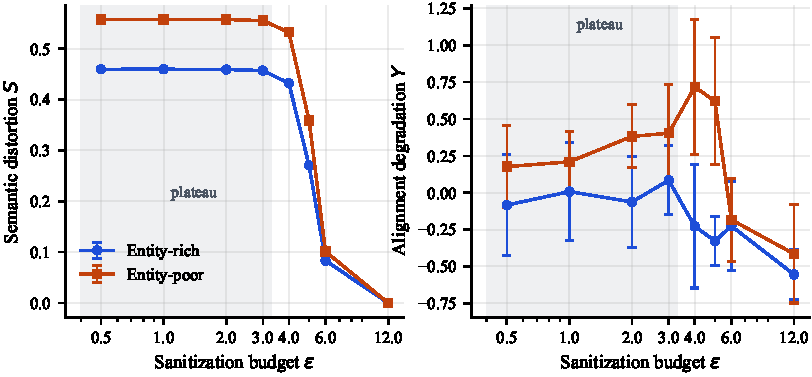
\includegraphics[width=0.78\linewidth]{threshold.pdf}
  \caption{\textbf{Half of the registered sanitization levels are behaviorally inert.} \textbf{Left:} distortion of the sanitized text against the budget.
  \textbf{Right:} the resulting degradation,
  error bars over three seeds.
  The shaded band is the plateau,
  $\varepsilon \le 3$,
  where distortion varies by $0.003$;
  the transition falls in $\varepsilon \in [4,
  6]$ and can be located from the distortion curve alone,
  before training anything.}
  \label{fig:threshold}
\end{figure}


\end{document}
